\chapter{Applications}

This section provides practical examples through which this extension shows itself to be useful and relevant in fulfilling its purpose of detecting vulnerabilities in websites. Firstly, we will demonstrate how the \textit{Recommendations} feature can be used as a low effort entry point into analysing websites for potential vulnerabilities. Secondly, we will use our Test Harness to demonstrate the uses of the \textit{Action Replay} feature in tweaking and replaying innocent requests to produce behaviour that exposes vulnerabilities on a website. We then show how the \textit{Passive Mode} behaves by showcasing how it performs against the intentionally vulnerable test page. Each of these sections will begin with a preamble covering how the example we will go through is vulnerable to establish a better understanding on how the extension exposes said vulnerability. Finally, we run through a case study of a live website vulnerability that we discovered and exploited as a result of using the extension on it.

\section{Recommendations} \label{applications_recommendations}

In order to set up the example to demonstrate a use case of the \textit{Recommendations}, we set up the Test Harness with 2 intentional XSS Vulnerabilities that work in the same way - any input that is submitted in either the \texttt{injection} or \texttt{injection2} input fields is reflected on the page below its respective input (in the \texttt{output} and \texttt{output2} fields respectively). The source code of the page at this point is shown in Listing \ref{lst:test_harness}, and the resulting rendered page is shown in Figure \ref{fig:test_harness_default}. \\


%\begin{minipage}{\linewidth}
\begin{lstlisting}[label={lst:test_harness}, language={HTML}, caption={The HTML contents of the Test Harness for this example. Two of the inputs in the page are reflected onto the page when they are submitted as query parameters (i.e. seen in the page URL)}]
<script>
	window.onload = function() {
		var url = new URL(window.location.href);
		
		var c = url.searchParams.get("injection");
		if (c) {
			document.getElementById("output").innerHTML = c;
		}
		
		var d = url.searchParams.get("injection2");
		if (d) {
			document.getElementById("output2").innerHTML = d;
		}
	}
</script>

<h1>Vulnerability Testing page</h1>

<form id="boop" action="">
	<input type="text" name="injection" value=""/>
	<input type="text" name="unused" value="">
	<input type="submit">
</form>
<h2 id="output"></h2>

<form id="beep" action="">
	<input type="text" name="unused" value=""/>
	<input type="text" name="injection2" value="">
	<input type="submit">
</form>
<h2 id="output2"></h2>
\end{lstlisting}
%\end{minipage}



\begin{figure}[h]
	\centering
	\begin{subfigure}{.45\textwidth}
		\centering
		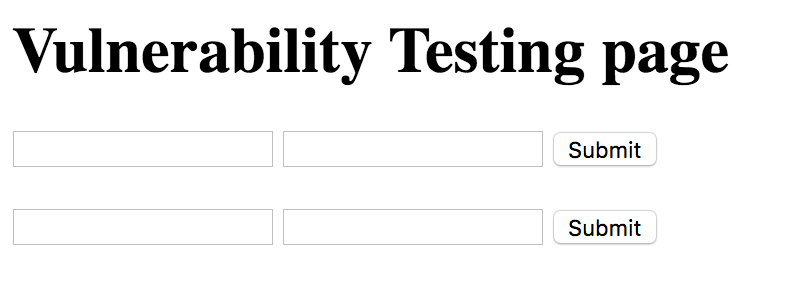
\includegraphics[width=.8\linewidth]{images/test_harness_recommendations.png}
		\label{fig:test_harness_original}
	\end{subfigure}%
	\begin{subfigure}{.6\textwidth}
		\centering
		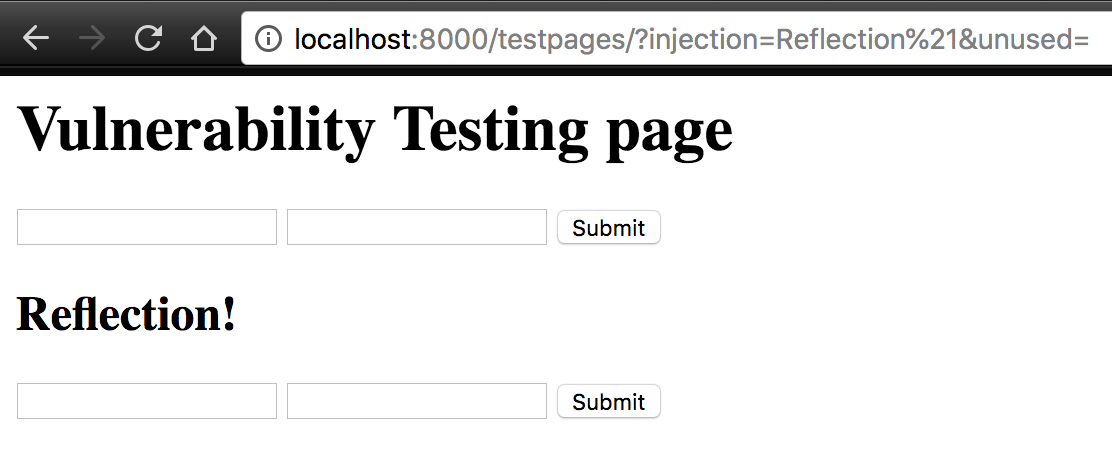
\includegraphics[width=.8\linewidth]{images/test_harness_reflection_1.png}
		\label{fig:test_harness_reflection_1}
	\end{subfigure}
	\caption{The default Test harness page to demonstrate XSS vulnerabilities. Submitting the first input causes the reflection in the second image.}
	\label{fig:test_harness_default}
\end{figure} 

Now we enable the recommendations in this page - setting the sensitivity parameter to \textbf{1}. At this stage, one input is added per form on the page, encouraging the user to "investigate" the first input on each of the forms, seen in Figure \ref{fig:test_harness_recommendations_2}. 

\begin{figure}[h]
	\centering
	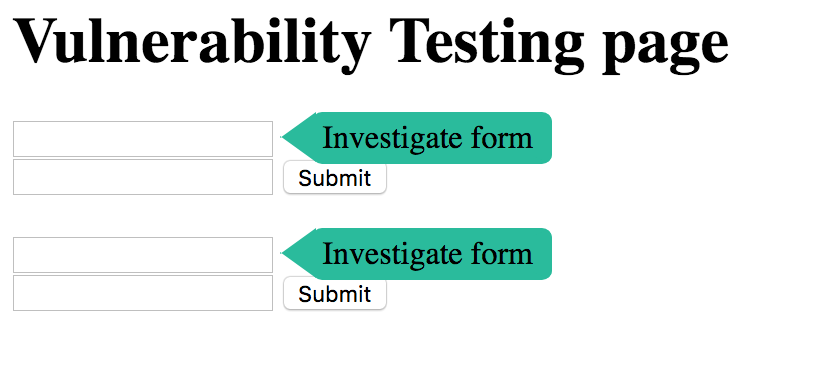
\includegraphics[width=0.7\textwidth]{images/test_harness_recommendations_2.png}
	\caption{Enabling the recommendations on the Test Harness}
	\label{fig:test_harness_recommendations_2}
\end{figure}

If the user decides to test the first input on the page, one of the attempted attacks will inject the following into the input:

\begin{center}
	\texttt{<img src=a onerror="window.location.replace( 'chrome-extension://ID/request\_logger.html?ref=CURRENT\_URL')">}
\end{center}

where the \texttt{ID} parameter is replaced by the ID given by Chrome to the extension, and the \texttt{CURRENT\_URL} is the current web address before the form was submitted. This is an example of an XSS attack which surreptitiously executes Javascript on a page by injecting an \texttt{<img>} tag with an invalid source location. This triggers an error when the image is later loaded on that page (since we have established that this input is reflected back onto the page). At this point, the \texttt{onerror} callback given to the input is executed, and in our case, will change the location of the current page to our previously mentioned \texttt{request\_logger} page, passing the current URL as a query parameter in this referral. \\


The \texttt{request\_logger} page is equipped to deal with this specific type of request, by alerting the user both through the extension and in the page output that an XSS vulnerability has been found, indicating the address of the culprit page. The only (current) means to reach this page in the extension is through the payloads prepared in the attacks, meaning that Javascript had to have been executed by one of these, thus indicating an XSS vulnerability. Upon opening the extension for further details, the initial Test Harness URL is then listed as a website vulnerable to XSS. \\


\begin{figure}[h]
	\centering
	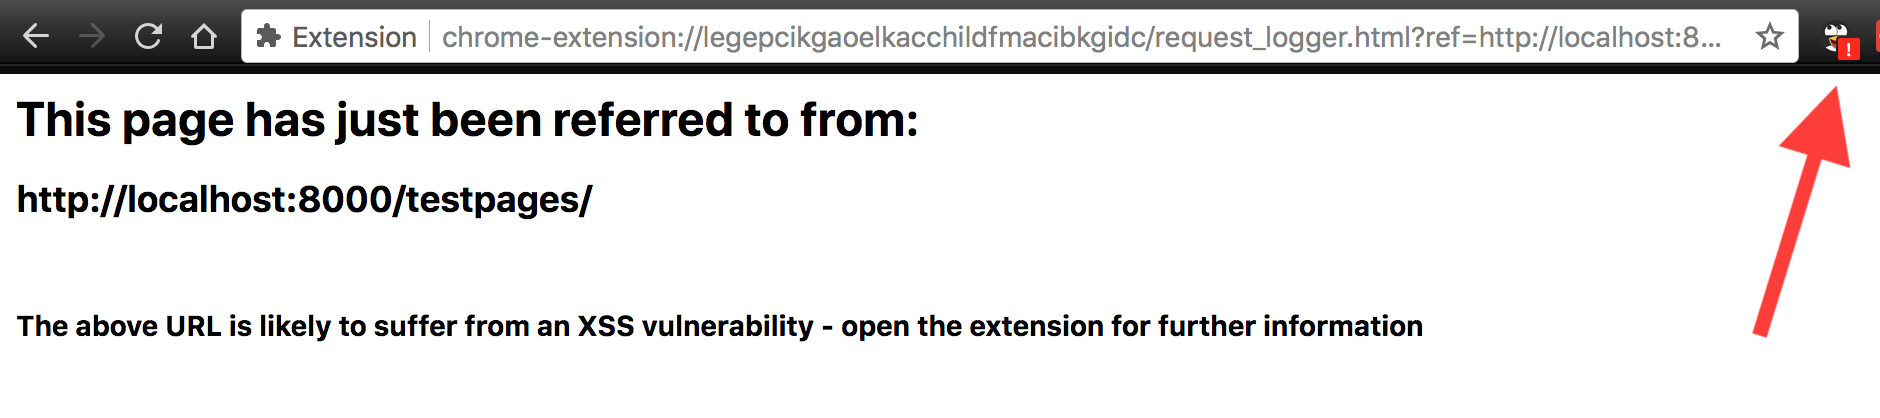
\includegraphics[width=	\textwidth]{images/request_logger_warning.png}
	\caption{The request logger page warns the user that the reason they've reached this page is likely to have been due to an XSS vulnerability. Note that the extension badge is also updated with a warning \textbf{(!)} label to indicate this (arrow added in diagram for emphasis).}
	\label{fig:request_logger_warning}
\end{figure}

\begin{figure}[h]
	\centering
	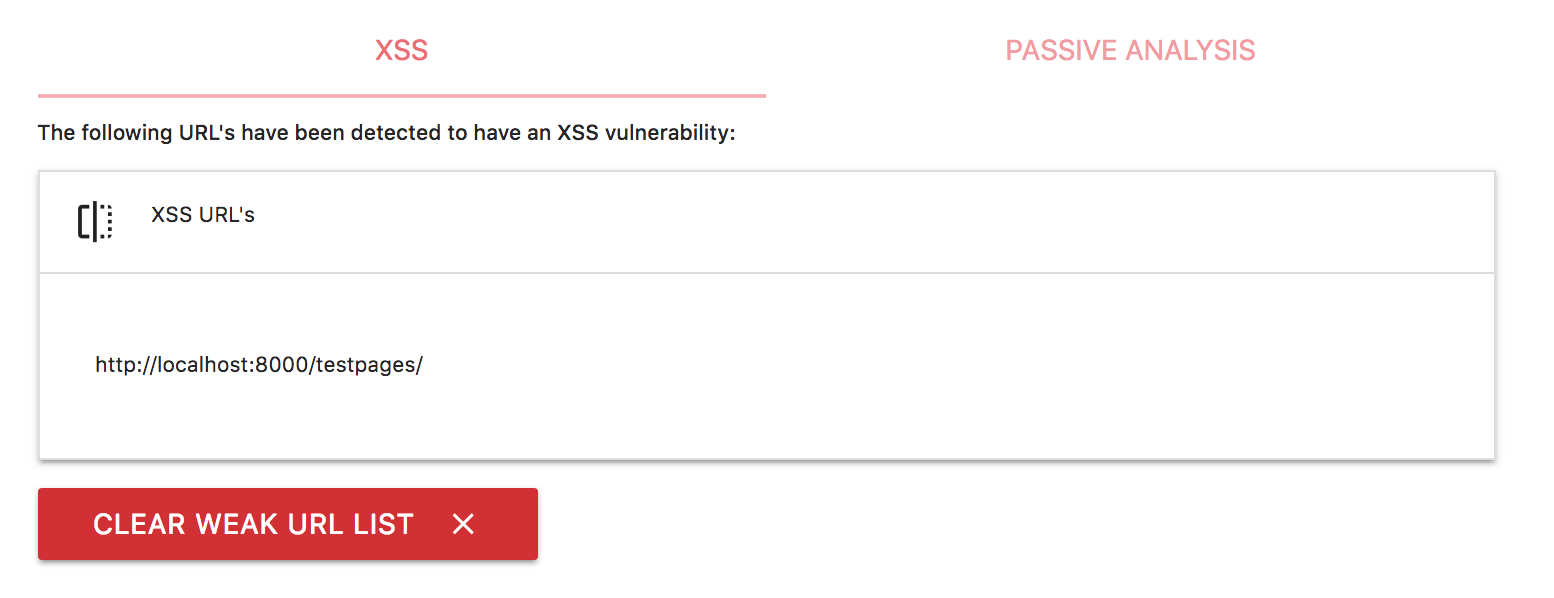
\includegraphics[width=	\textwidth]{images/xss_vulnerable_url.png}
	\caption{Opening the extension confirms that the suspicious URL was indeed vulnerable to XSS.}
	\label{fig:xss_vulnerable_url}
\end{figure}

However, this has only covered one of the vulnerabilities on the page - there is still another vulnerability in the last input on the page, which is reflected in the same way as above. However, clicking the second \textit{Investigate Form} button in this case will not reveal anything about the last vulnerable input - it will only attack the first input in the second form on the page. This attack results in nothing besides the submission of the second form and the reloading of the page. This emphasises the need for a Recommendation Sensitivity setting - if we change it from \textbf{1} to \textbf{2}, more suggestions are added to the page (1 for every \texttt{<input>} tag); we can now attack the last input. This results in a vulnerability detection process very similar to the one described above for the other input.   

\section{Action Replay}

Now we consider how we can use the Action Replay algorithm to automatically replay attacks on focussed inputs and requests. \\

The vulnerability in this example is the same as the one from the \textit{Recommendations} section (\ref{applications_recommendations}) - the website suffers from a reflected XSS vulnerability. Here, we assume that through use of the website, the user has noticed there may be a vulnerability present, and attempts to exploit the website. Perhaps they attempt a similar injection as before to test their hypothesis:

\begin{center}
	\texttt{<img src=a >} 
\end{center}

Upon trying this input, they are confronted with the page shown in Figure \ref{fig:action_replay_initial}. \\

\begin{figure}[h!]
	\centering
	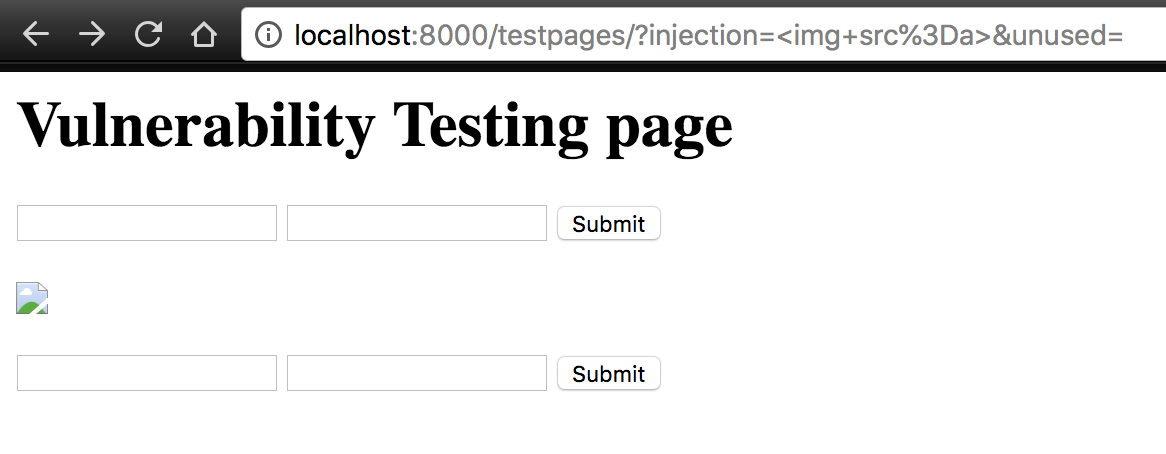
\includegraphics[width=0.7\textwidth]{images/action_replay_initial.png}
	\caption{Injecting \texttt{<img src=a>} into an input results in this page}
	\label{fig:action_replay_initial}
\end{figure}

To a web security analyst with a more trained eye, this may present a security risk, as they were freely able to inject a HTML tag into the page of their choosing. It is at this point where they decide to focus on this particular input and activate the Action Replay. After enabling and starting a recording, they reattempt the earlier injection (Figure \ref{fig:action_replay_attack}). \\

\begin{figure}[h!]
	\centering
	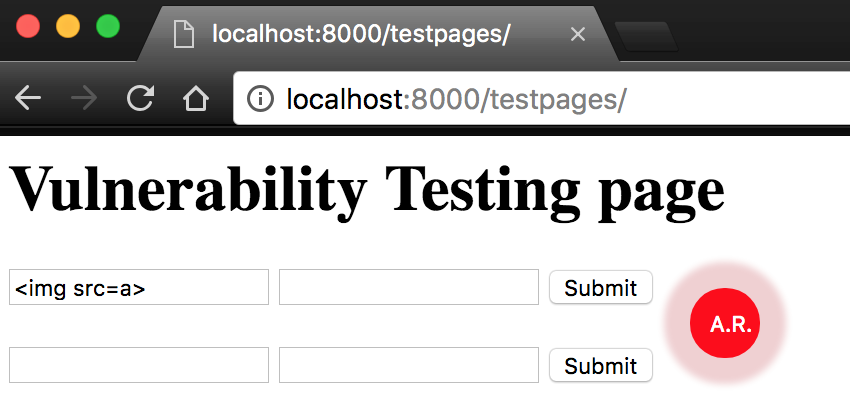
\includegraphics[width=0.7\textwidth]{images/action_replay_attack.png}
	\caption{Retrying the attack while recording using Action Replay}
	\label{fig:action_replay_attack}
\end{figure}

Once the new page loads, the user can then stop the recording by clicking the \textit{AR} button once again. At this point, the analysis and automated replay begins. If the algorithm has appropriately detected a set of potentially dangerous inputs it can override to begin an attack, then almost immediately after finishing the recording, Chrome will open several new windows, each of which attempts an attack. Not all of these are expected to yield successful vulnerability identifications, but, for this example, we see that one of the resultant tabs has ended up in the \textit{Request Logger} page. This can only indicate that the payload of one of the attacks was successful (Figure \ref{fig:successful_replay}). \\ 


\begin{figure}[h!]
	\centering
	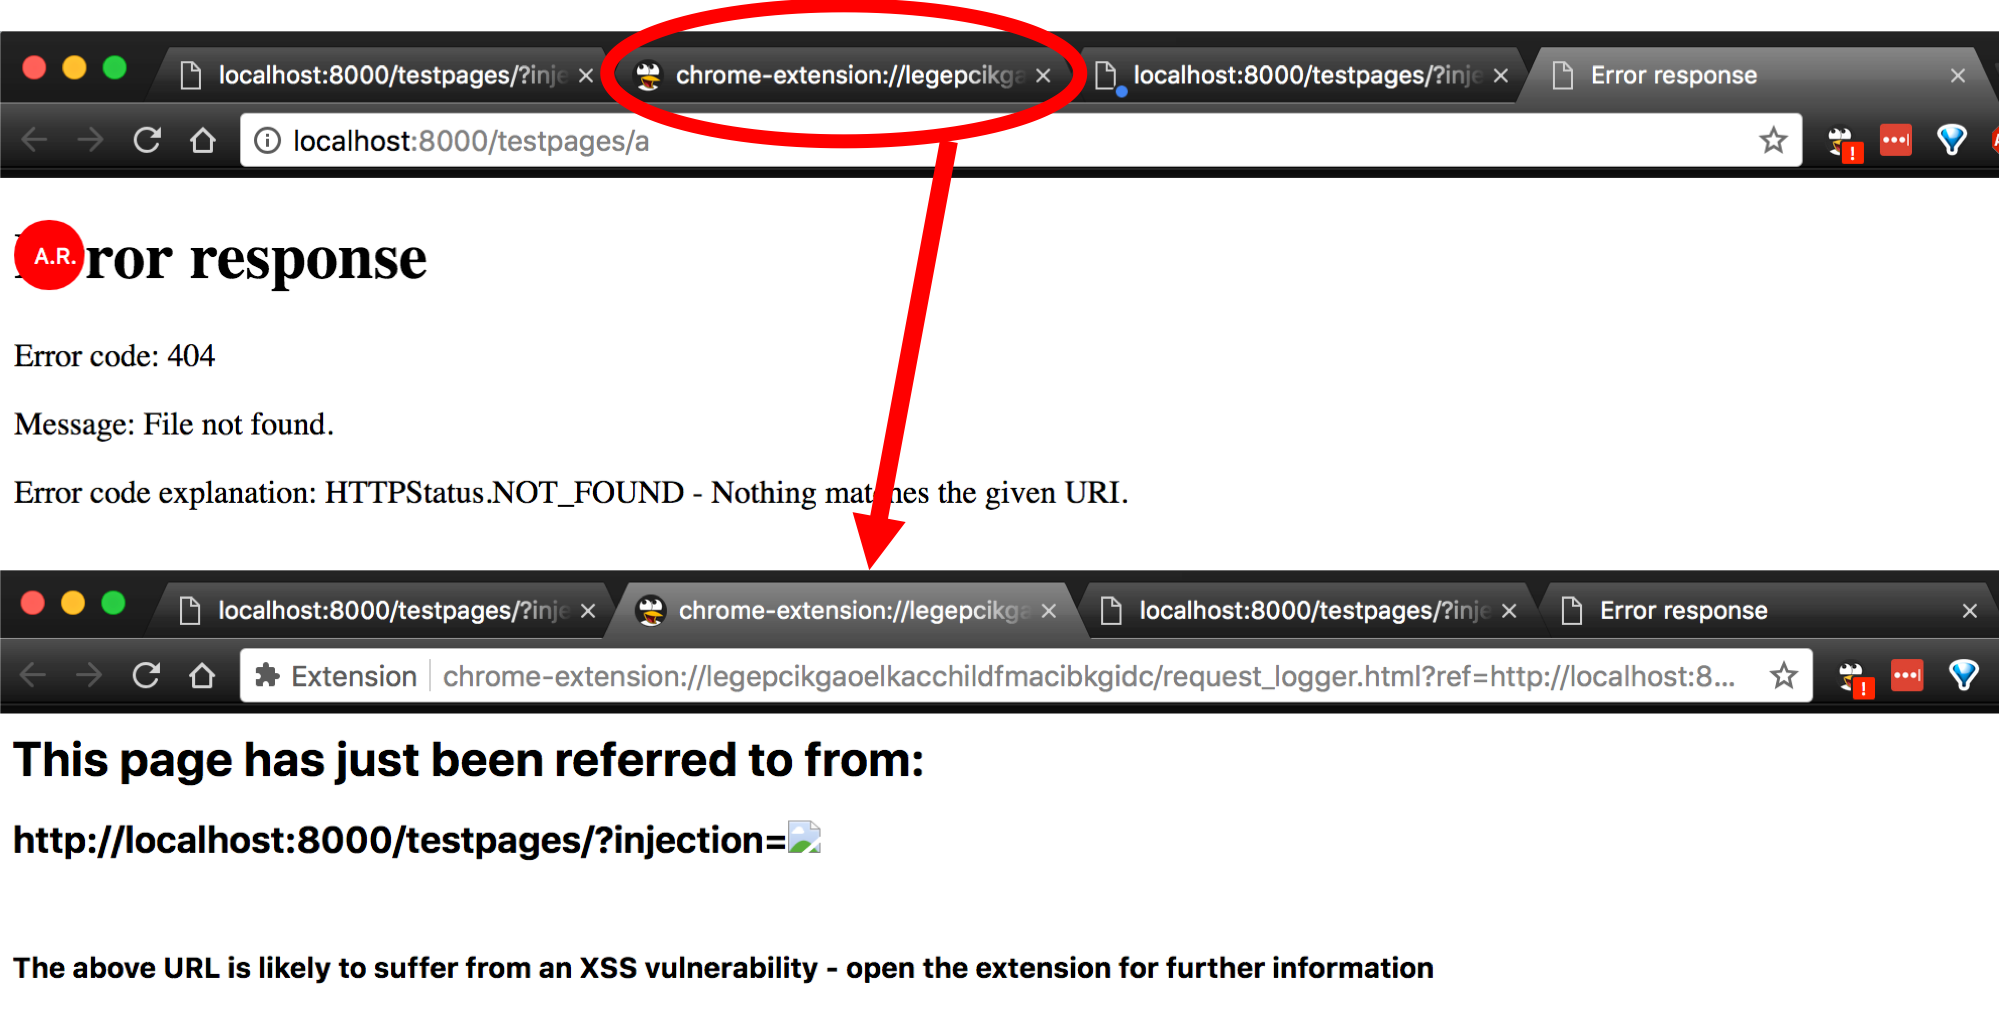
\includegraphics[width=\textwidth]{images/successful_replay.png}
	\caption{The Action Replay generates the outputs of several attacks in new windows. The 2nd of the inspected windows showcases a successfully detected vulnerability that executed a Javascript payload.}
	\label{fig:successful_replay}
\end{figure}

As before, once this stage is reached, we have the appropriately reported information in the extension. The list of URLs that suffer from XSS vulnerabities is updated, containing the latest victim. Additionally, Action Replay publishes a list of inputs it considered to be dangerous, showing the user which inputs were targeted by the automated attacks (Figure \ref{fig:dangerous_inputs}).  \\

\begin{figure}[h!]
	\centering
	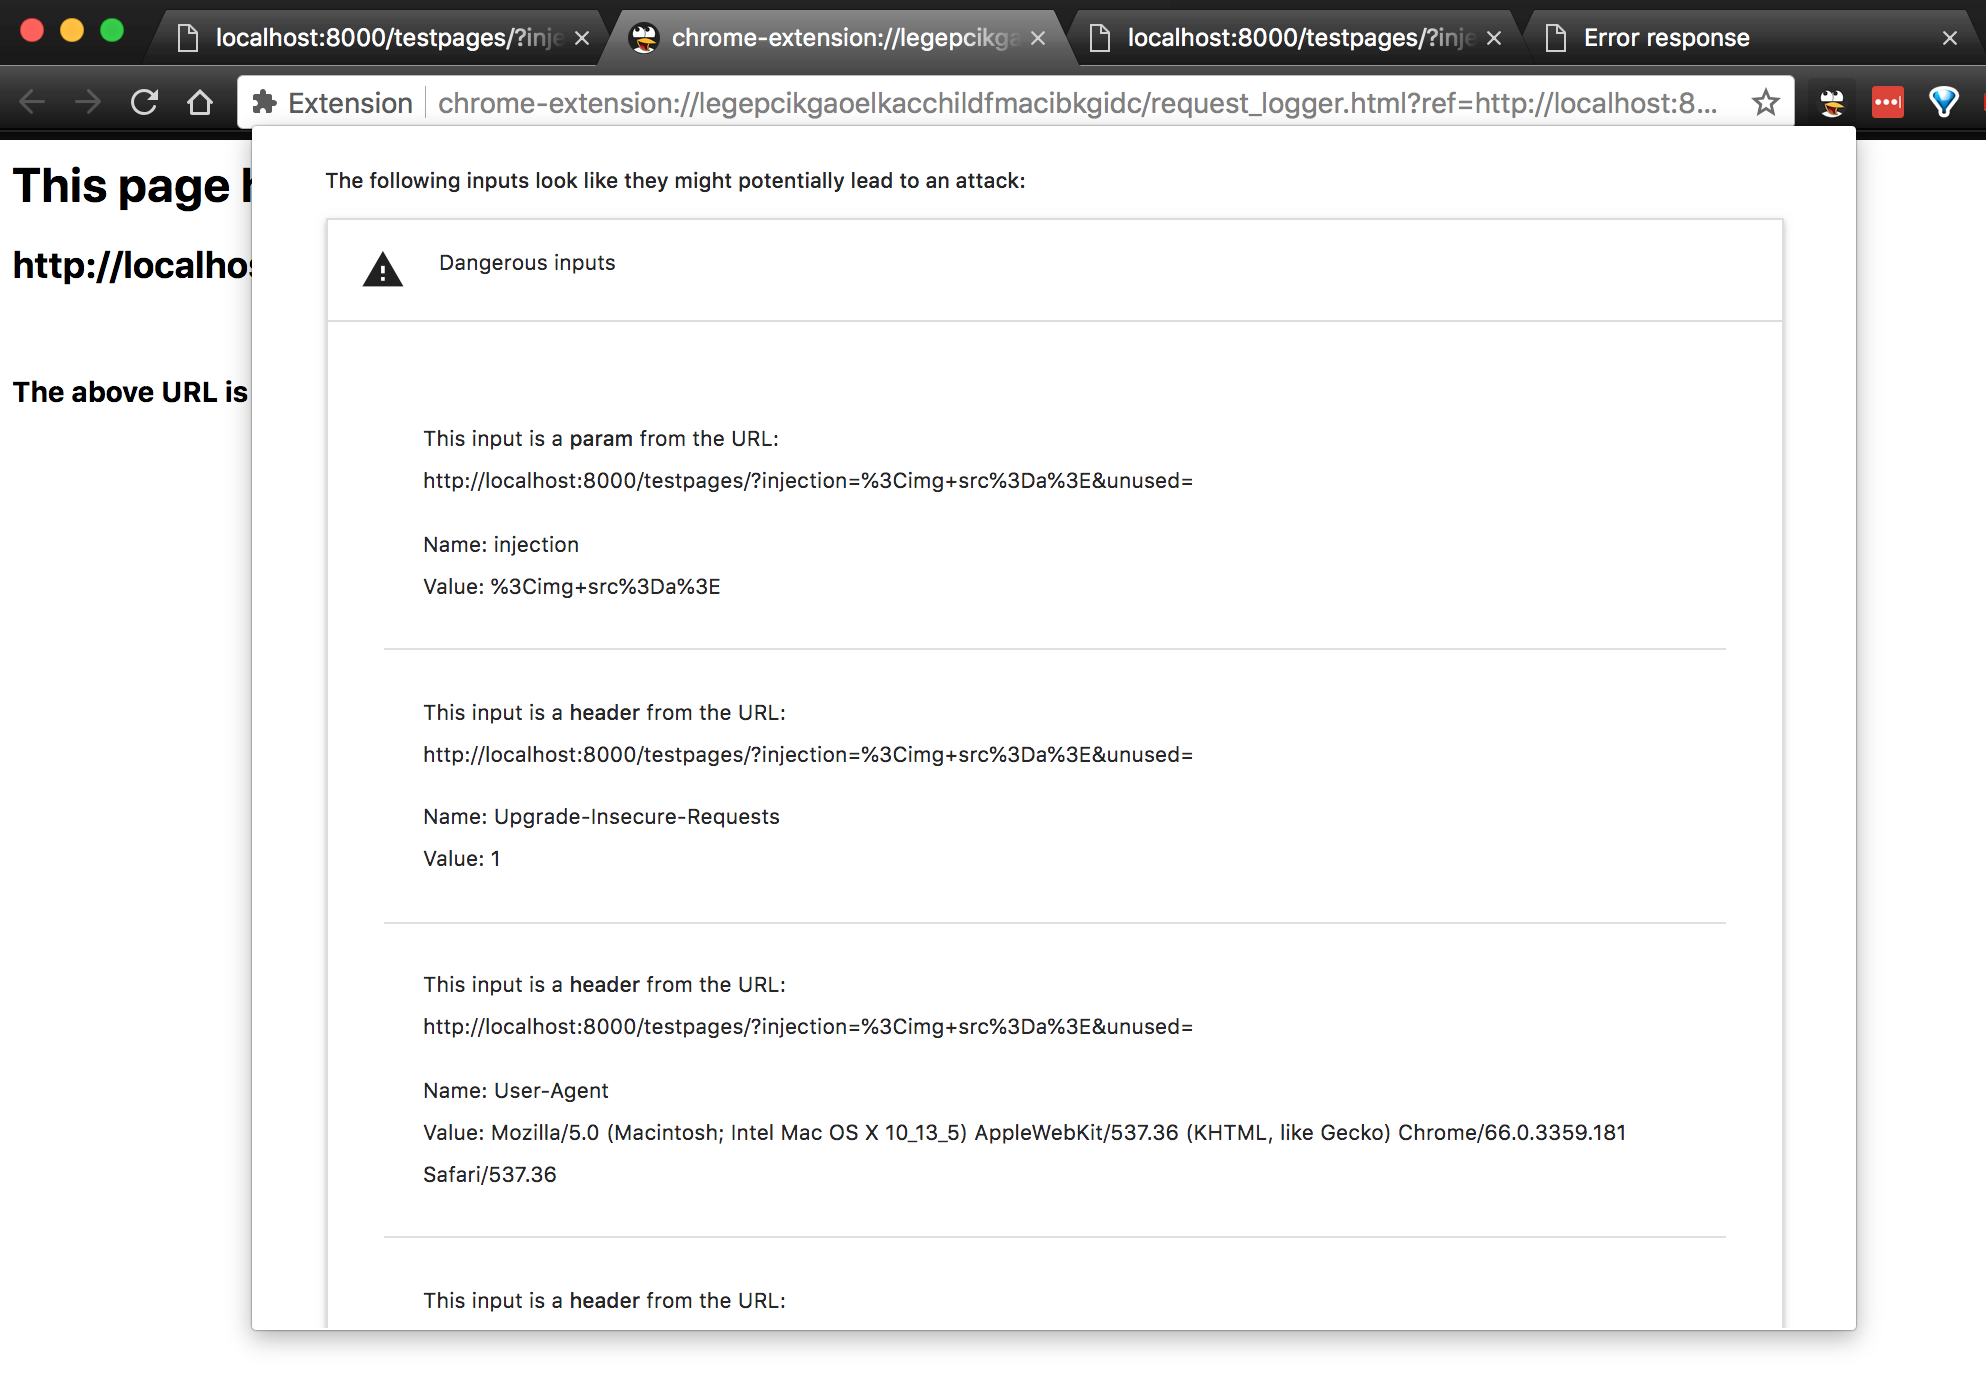
\includegraphics[width=\textwidth]{images/dangerous_inputs.png}
	\caption{The Action Replay outputs a list of inputs it has considered to be dangerous. In this screenshot, we see the \textbf{param} with the name \textbf{injection} is one of the potentially dangerous inputs. }
	\label{fig:dangerous_inputs}
\end{figure}

\section{Passive Mode}

We now review the Passive Mode and highlight what useful information it can produce to a user while they use the website in a normal fashion. By default, this mode will check that a set of headers are being sent with each request and response. To demonstrate a worst case scenario of an insecure site, we make no intentional changes to the Test Harness page. As expected, this raises warnings for all of the headers enumerated in section \ref{header_analysis}. The outputs of this scan are shown in Figure \ref{fig:passive_weak_headers_1}. \\

\begin{figure}[h!]
	\centering
	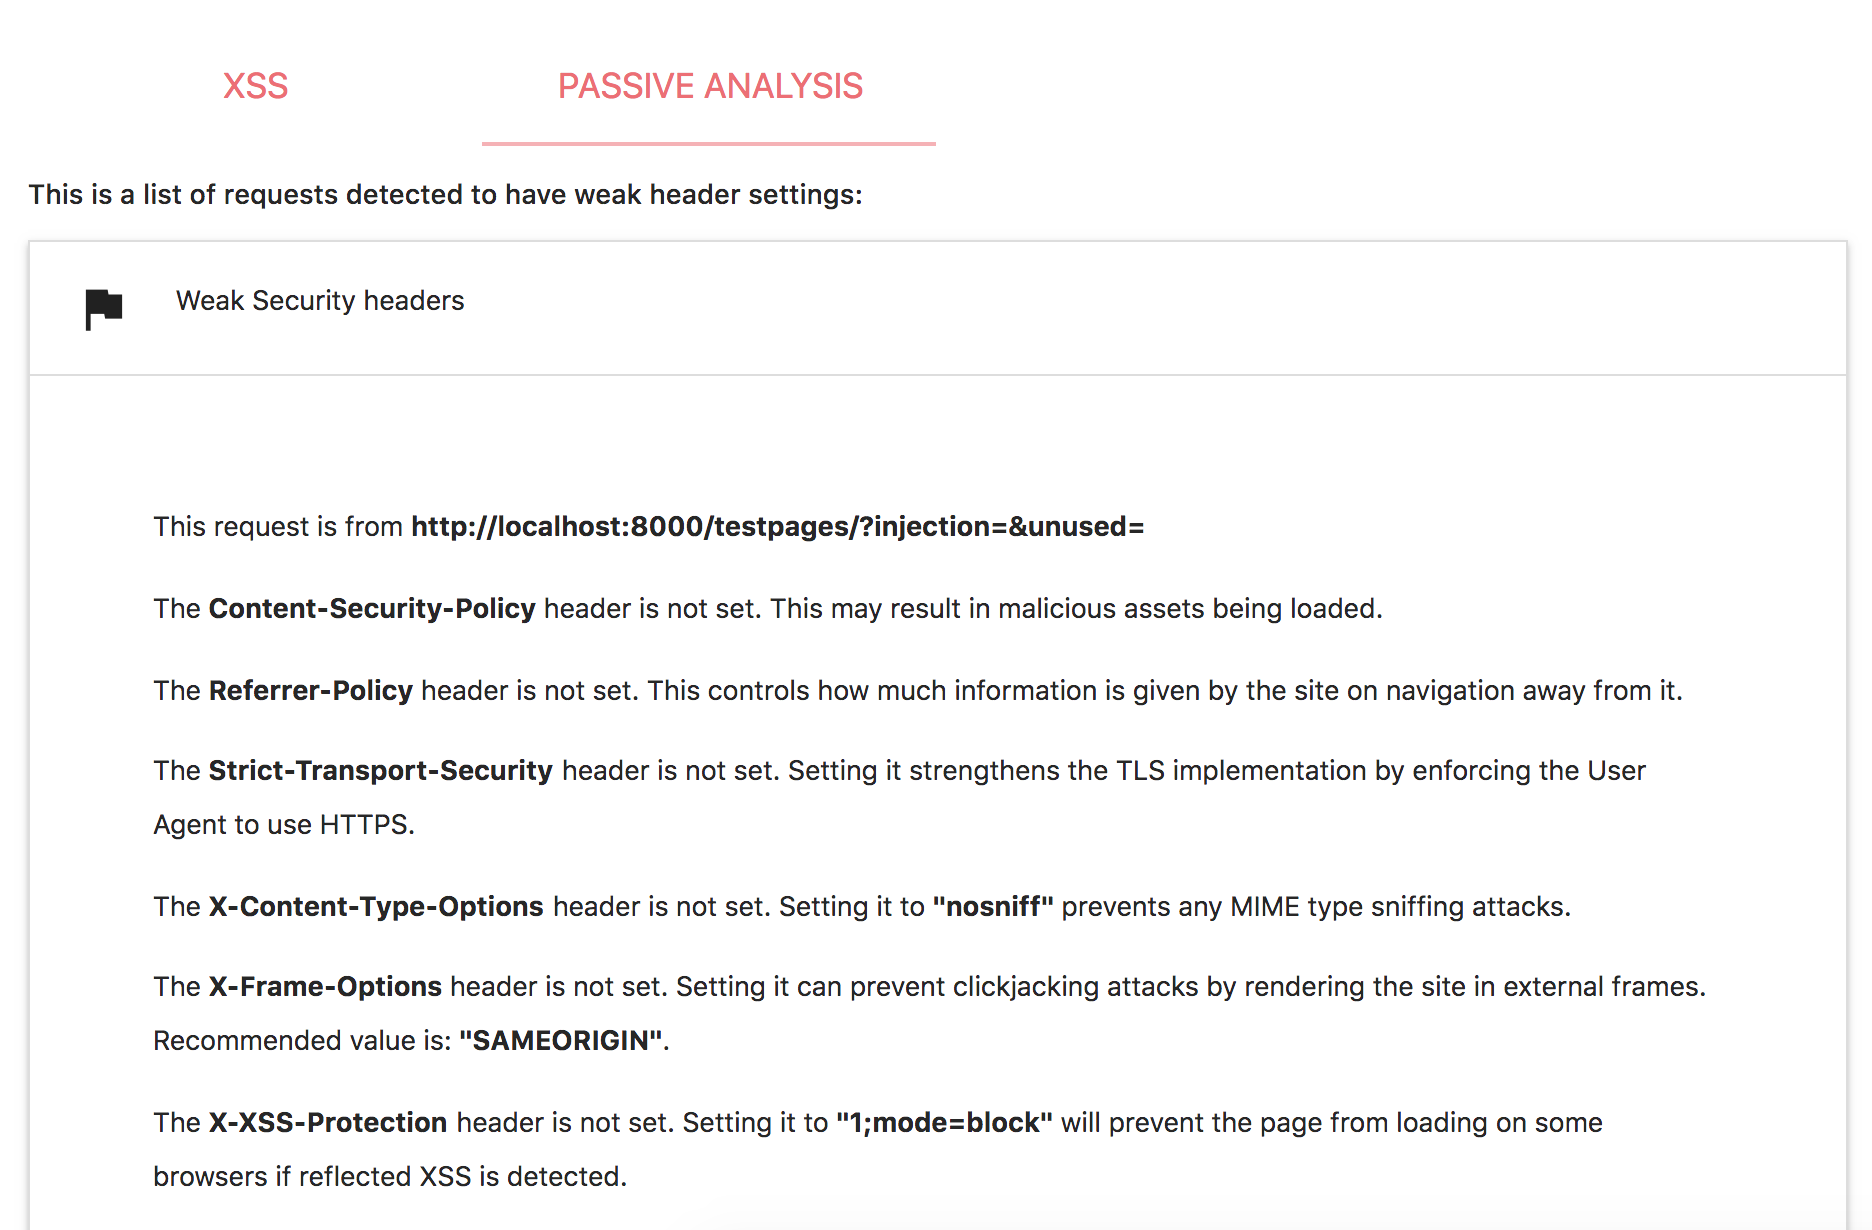
\includegraphics[width=\textwidth]{images/passive_weak_headers_1.png}
	\caption{A webpage which makes no effort to set secure headers (as the Test Harness does here) will raise up warnings by the passive mode in this regard.}
	\label{fig:passive_weak_headers_1}
\end{figure}

If we scan another website however, we are more likely to find a bit more attention to detail in terms of setting secure headers. We scanned \url{http://google.com} and came up with better results than the Test Harness - at least half of these headers had been set to their recommended settings as shown in Figures \ref{fig:google_headers} and \ref{fig:google_headers_2}. \\

\begin{figure}[h!]
	\centering
	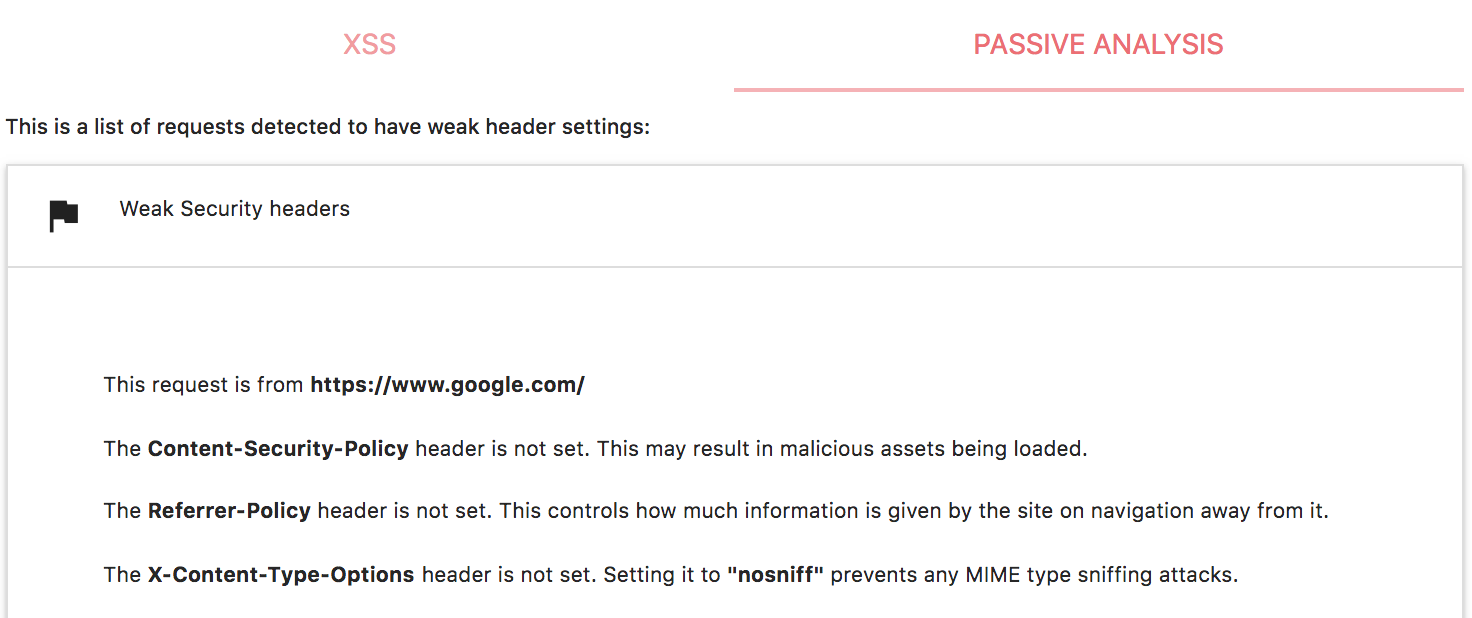
\includegraphics[width=\textwidth]{images/google_headers.png}
	\caption{The header analysis from scanning \texttt{http://google.com} shows that some of the security headers have been set, but others are still unset.}
	\label{fig:google_headers}
\end{figure}

\begin{figure}[h!]
	\centering
	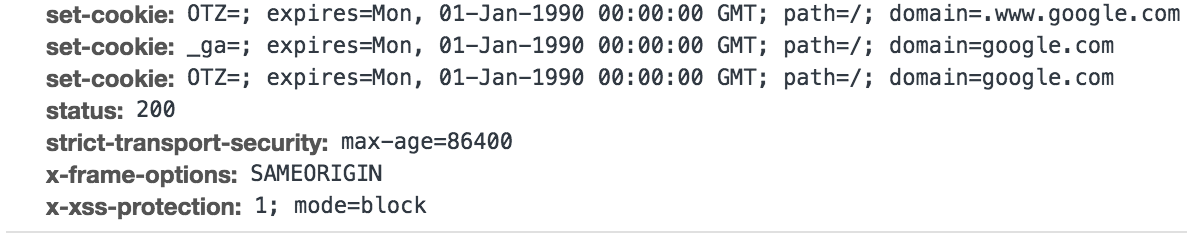
\includegraphics[width=\textwidth]{images/google_headers_2.png}
	\caption{Looking at the request details in the Developer Tools in Chrome reveals that the headers that were not reported by the extension had been set by Google.}
	\label{fig:google_headers_2}
\end{figure}

Besides headers, this mode also checks for potentially reflected user-controlled inputs (much like the Action Replay algorithm). Here we reuse the vulnerabilities from the Test Harness page as a means to test the outputs of this algorithm. As before, we submit the first input, which we know to be reflected on submission. This appends a warning to the log produced for this request, as shown in Figure \ref{fig:passive_reflection}.

\begin{figure}[h!]
	\centering
	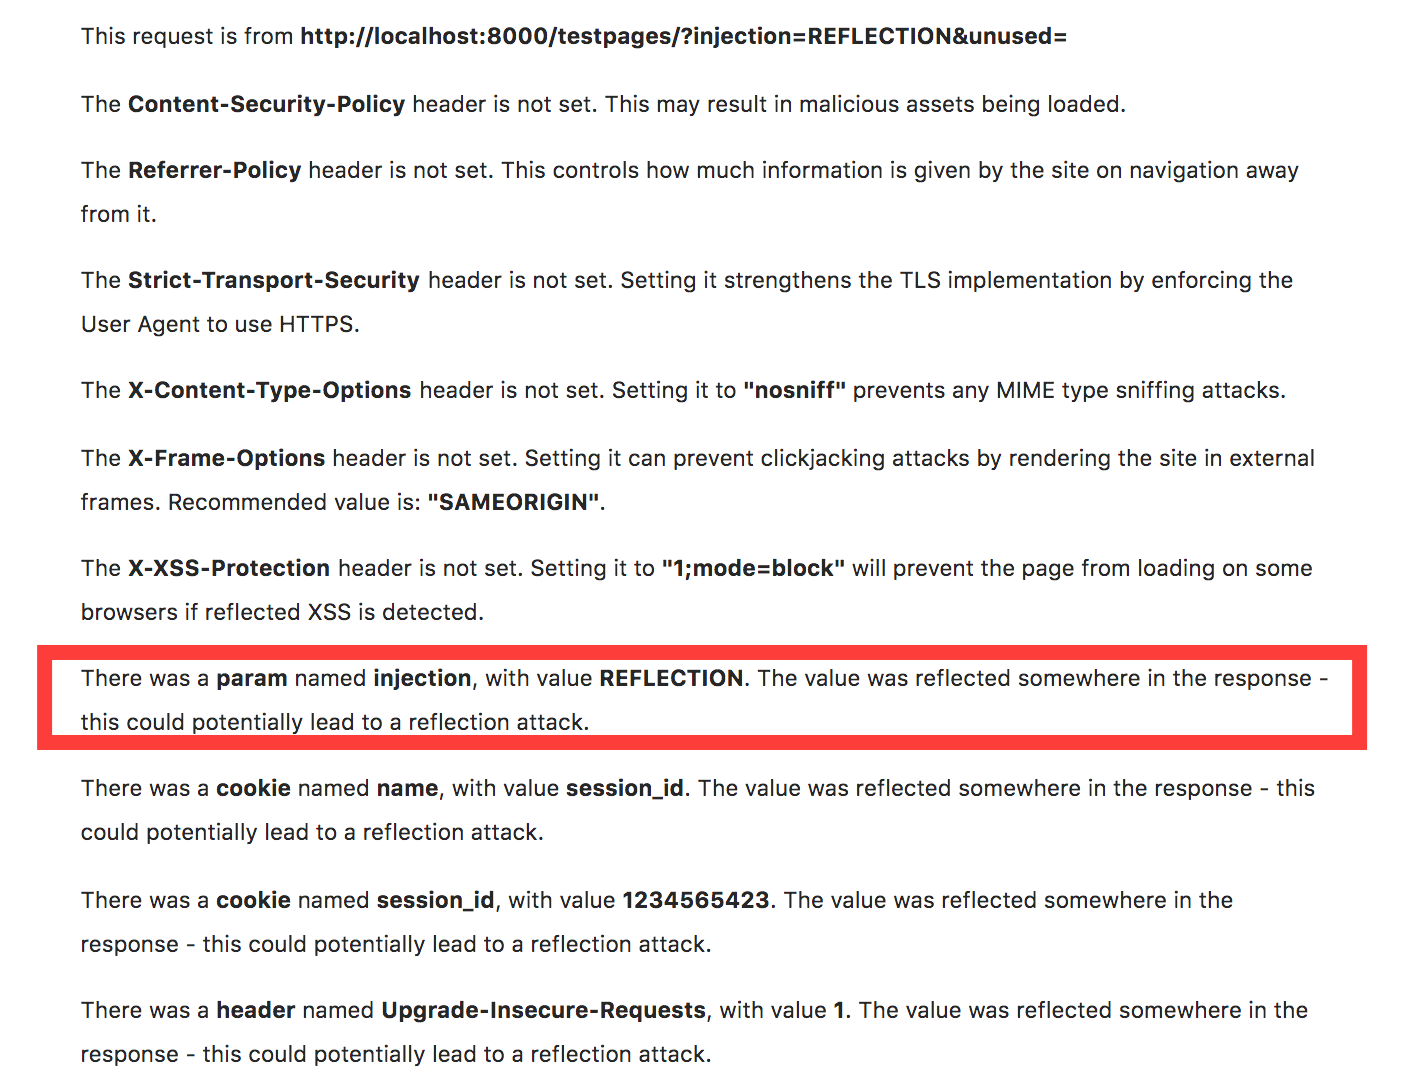
\includegraphics[width=\textwidth]{images/passive_reflection.png}
	\caption{Although this mode is liberal in highlighting potential vulnerabilities, amidst the warnings we see that it has detected the reflected input caused by the query parameter.}
	\label{fig:passive_reflection}
\end{figure}


\subsection{CSRF alerts} \label{applications_CSRF_alerts}

As explained in Section \ref{csrfChecks}, this mode is also equipped to perform some basic checks to alert the user to factors which may facilitate the crafting of CSRF attacks, as long as the correct setting is enabled. To emulate this situation, we add some cookies to the Test Harness using Javascript. One of these is purposefully named with keywords that will trigger our filter that looks for cookies that store session IDs. We add the code in Listing \ref{lst:csrf_cookies} to the Javascript portion of our page.

\begin{lstlisting}[label={lst:csrf_cookies}, language={HTML}, caption={We add some cookies to the page - one of these is designed to trigger our filter to find Session ID related cookies}]
...
<script>
	window.onload = function() {
		...
		document.cookie = "fake_cookie_1=BOOP;"
		document.cookie = "session_id=1234565423";
		document.cookie = "analytics_cookie=BEEP";
	}
<script>
...
\end{lstlisting}

The rest of our Test Harness page already fulfills the minimum requirements for the CSRF alert - it contains forms but none of these are equipped with a hidden \texttt{<input>} tag (which would be expected to be used as an Anti-CSRF token, given that it has a session cookie). This results in the CSRF alert being produced for this page as shown in Figure \ref{fig:csrf_warning}.

\begin{figure}[h!]
	\centering
	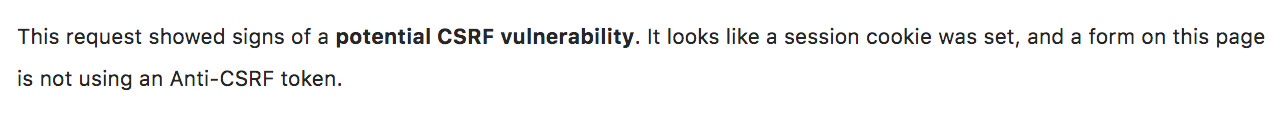
\includegraphics[width=\textwidth]{images/csrf_warning.png}
	\caption{When the website conforms to the minimum requirements previously explained, the passive analysis produces this CSRF warning.}
	\label{fig:csrf_warning}
\end{figure}

\subsection{Insecure Cookie Alerts}

Passive mode can also check whether any potentially important or valuable cookies are being set with the appropriate security settings. Setting up an example to demonstrate this is the same as described in Section \ref{applications_CSRF_alerts} - we will reuse the same 3 cookies for this case. The only seemingly \textit{valuable} cookie in this case is the same, the one that stores the "session\_id" for the user. Only this cookie should raise any alerts about not being set securely. This is what we see shown in Figure \ref{fig:cookie_warning}. As expected, setting one or both of these flags in the cookie will change or delete the warning altogether.  \\

\begin{figure}[h!]
	\centering
	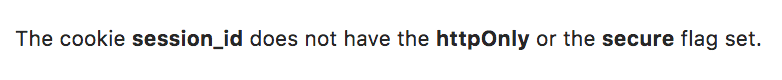
\includegraphics[width=0.85\textwidth]{images/cookie_warning.png}
	\caption{The extension warns of any cookies that may be of particular value to the user experience (such as the session ID) and have not been set with the appropriate security flags.}
	\label{fig:cookie_warning}
\end{figure}



\subsection{Request Cross Checks}

Now we showcase the cross check feature at work. This component has the ability to detect patterns that manifest themselves an arbitrary amount of requests apart. It is designed to find second-order attacks, but we will simulate this in a simpler way - we take advantage of the reflection vulnerability in our test harness to analyse outputs across different requests. In order to demonstrate a convincing enough example of the algorithm at work, we adopt the following strategy:

\begin{enumerate}
	\item After setting up the extension to analyse cross requests, we set the window size to a value of 3. This gives us enough separation to analyse outputs with at least one "uncorrelated" request inbetween.
	
	\item We submit the first form of the Test Harness using both inputs - we use the reflected input as the ongoing vulnerability, and we use the previously \texttt{unused} input in the form to keep track of what request we are on. For the purpose of this example, we submit the \texttt{injection} parameter with the value \texttt{BLUE} and the \texttt{unused} parameter with the value \texttt{Number 1} (as it is our first request).
	
	\item On the resulting page, we now submit the same form using different values for the same inputs - the \texttt{injection} parameter will be \texttt{RED} and the \texttt{unused} parameter will be \texttt{Number 2}.
	
	\item The algorithm generates several pages as a result of comparisons (this is necessary to obtain the resulting output of running the Javascript code that causes the reflections). We select one of these pages and now submit the form with \texttt{injection} to be \texttt{BLUE} again (hence replicating the behaviour of being our "second-order vulnerability") and the \texttt{unused} input as \texttt{Number 3} (as it is our final request).
\end{enumerate}

This strategy should be sufficient to demonstrate an example that showcases the cross request comparison. After executing this, we find the desired results - amongst several other warnings due to a large number of comparison, the extension points out that the \texttt{BLUE} value as seen in the third request (the one where the \texttt{unused} parameter was \texttt{Number 3}) had been already seen as a parameter value back in the first request. A partial screenshot of the results is shown in Figure \ref{fig:cross_check_warnings}. This demonstrates the capacity of using some directed automated techniques to analyse data which may otherwise seem distant; finding this sort of vulnerability with a much larger request window size would be more 

\begin{figure}[h!]
	\centering
	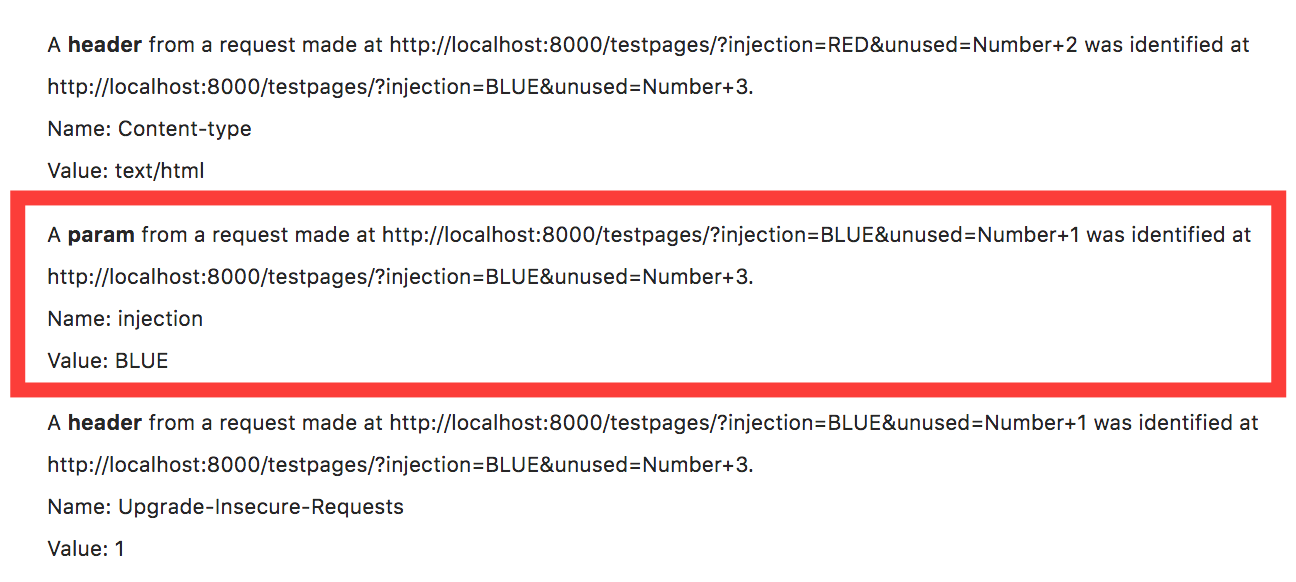
\includegraphics[width=0.85\textwidth]{images/cross_request_warnings.png}
	\caption{The extension finds the reflected exploit across requests with a separating distance of at least 1 other request. The image omits a substantial amount of other warnings.}
	\label{fig:cross_check_warnings}
\end{figure}


\section{Live Vulnerability Test Case} \label{live_vulnerability}

This section will describe a series of steps taken while using the extension that lead to the discovery of a real vulnerability on a live website. As part of the section we will demonstrate how this vulnerability can further be exploited. The website belongs to a fitness organization based in India; the specific login page we will consider is regularly used by over 1000 gyms / fitness studios. According to \url{alexa.com},\footnote{Not to be confused with Amazon's voice assistant, although both services are owned by Amazon.} this login form accounts for approximately 27\% of the traffic on the main domain. The website is kept anonymous as a courtesy to its rightful owners; in the meantime, the vulnerability has also been responsibly closed to the owners of the website. \\ 

This particular vulnerability was discovered as a result of using the recommendations feature of the extension. Figure \ref{fig:vuln_page} shows the login form before and after enabling the recommendations in the extension, at a sensitivity of \textbf{2}.

\begin{figure}[h]
	\centering
	\begin{subfigure}{.5\textwidth}
		\centering
		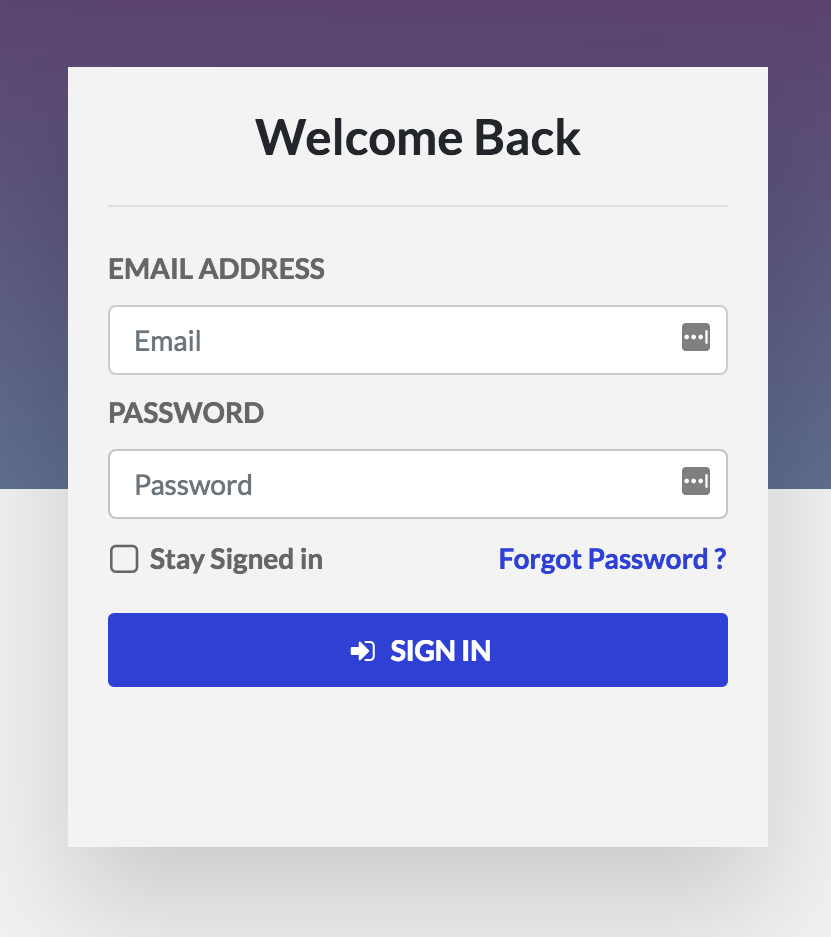
\includegraphics[width=.8\linewidth]{images/test_case_1/original_page_anon_cropped.png}
		\label{fig:original_page_anon}
	\end{subfigure}%
	\begin{subfigure}{.5\textwidth}
		\centering
		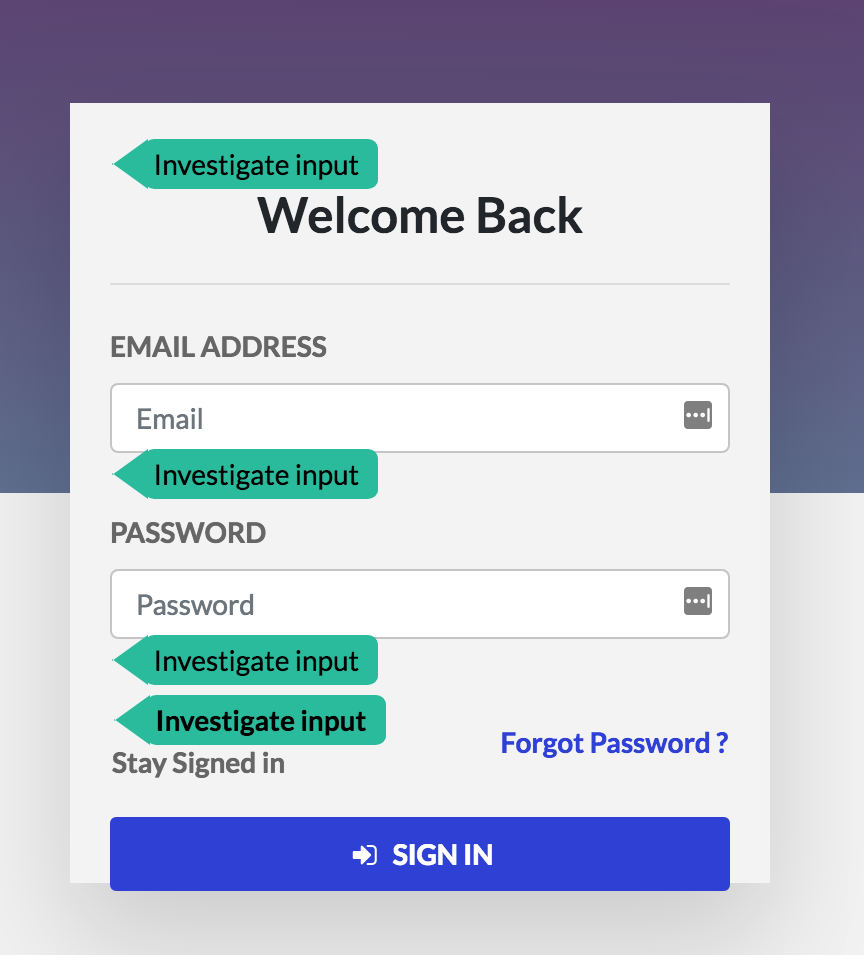
\includegraphics[width=.8\linewidth]{images/test_case_1/recommendations_anon_cropped.png}
		\label{fig:recommendations_anon}
	\end{subfigure}
	\caption{Here we see the website form before and after having the \textit{Recommendations} setting enabled. We see that it highlights both normal inputs in the form, as well as a hidden input, shown by the \textit{Investigate Form} button floating above the "Welcome Back" text.}
	\label{fig:vuln_page}
\end{figure} 

We decide to "investigate" the email input further - by clicking the button it automatically submits the form using an attack from those preprogrammed in the extension. The attack we submit at this time is an XSS attempt by trying to inject an image whose \texttt{onerror} property is triggered due to a faulty image source. Attempting this injection gives us the output shown in Figure \ref{fig:trigger_point}. \\

\begin{figure}[h!]
	\centering
	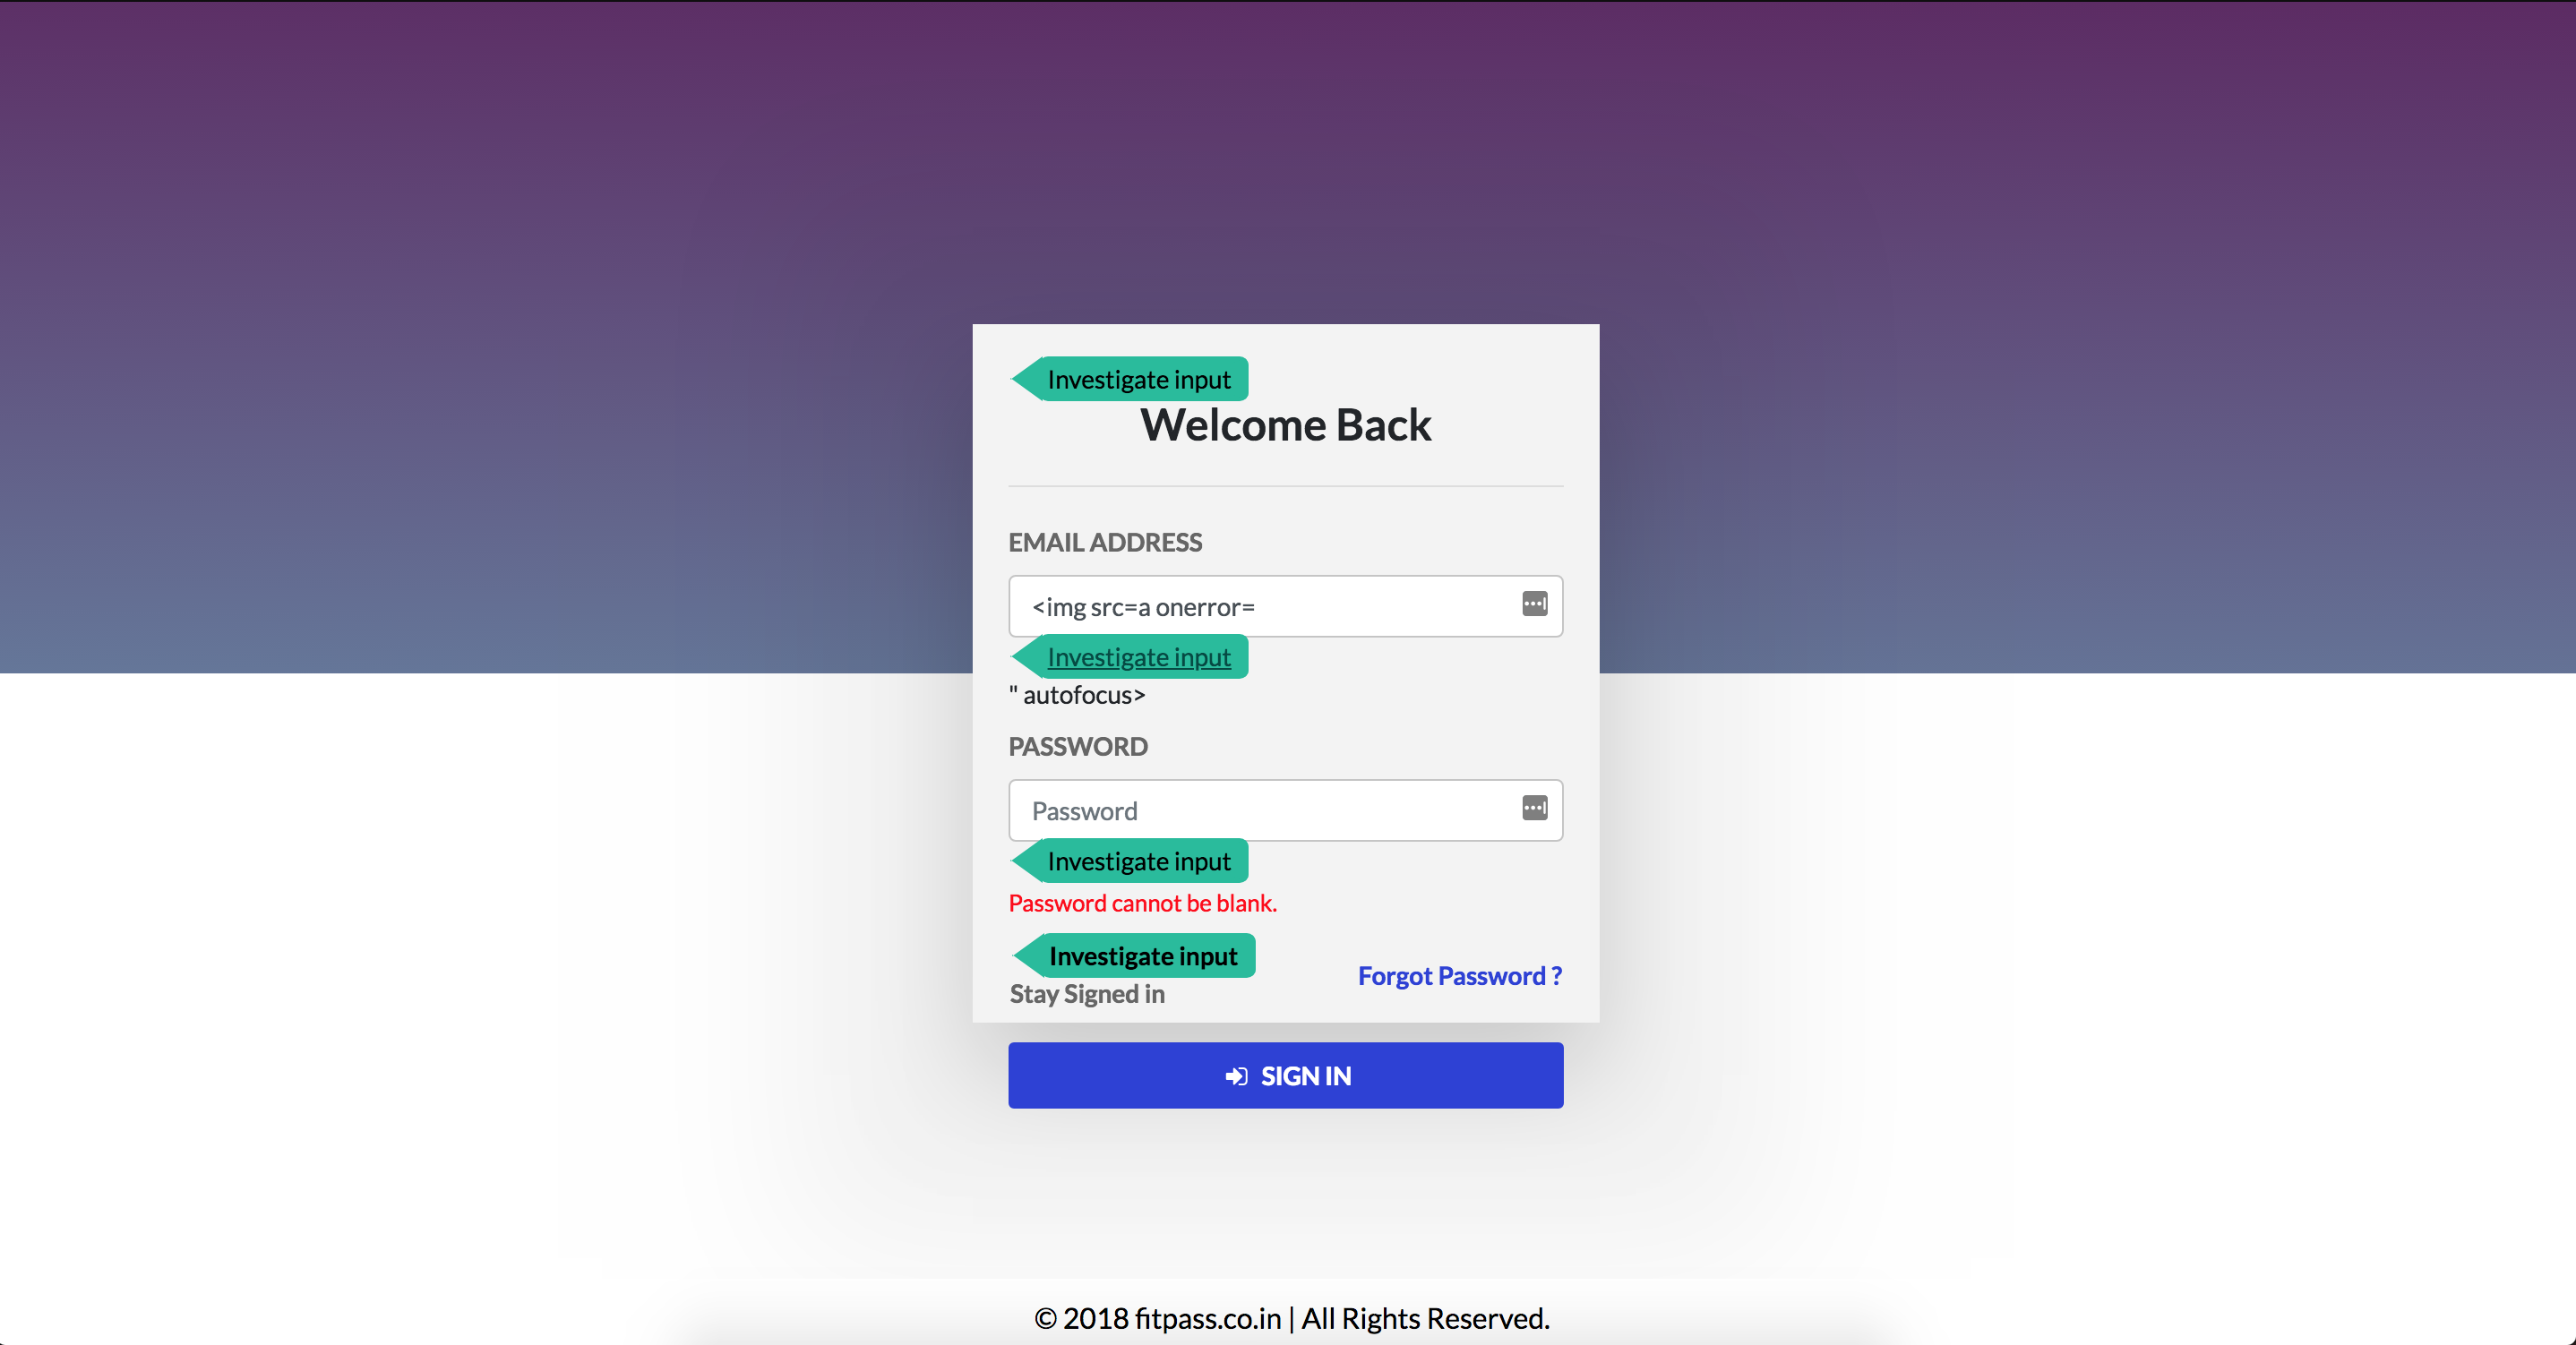
\includegraphics[width=0.75\textwidth]{images/test_case_1/trigger_point_anon.png}
	\caption{Here the form returns an error with a warning saying that the \textit{Password can't be blank}. However, this is not the interesting behaviour - we instead notice the presence of the following text after the Email address input: \texttt{" autofocus>}. This wasn't there before, and is not part of the attack.}
	\label{fig:trigger_point}
\end{figure}

This behaviour is interesting because the form has now added the text \texttt{" autofocus>} onto the form. This text was not previously in the login form; neither before or after adding the recommendations onto the page, so it must have been added as a result of submitting the attack on the form. To confirm this, we can check the source code of the page before and after the attack. 

\begin{figure}[h!]
	\centering
	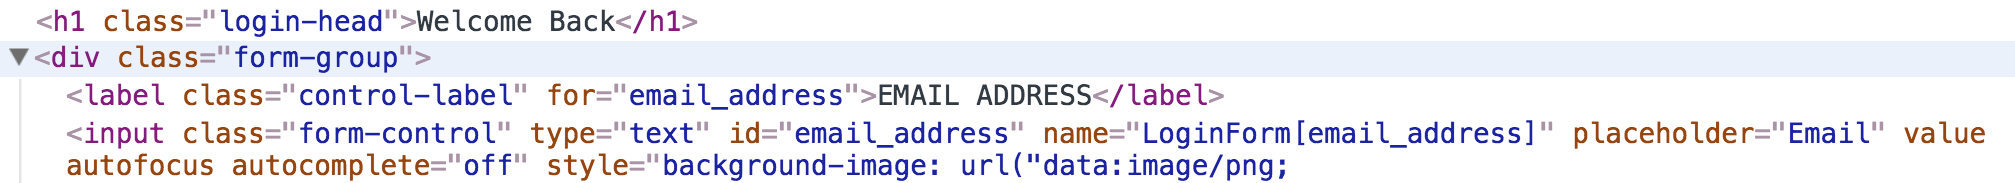
\includegraphics[width=\linewidth]{images/test_case_1/src_code_before.png}
	\caption{The source code of the login form before adding the recommendations or submitting an attack.}
	\label{fig:src_code_before}
\end{figure}

\begin{figure}[h!]
	\centering
	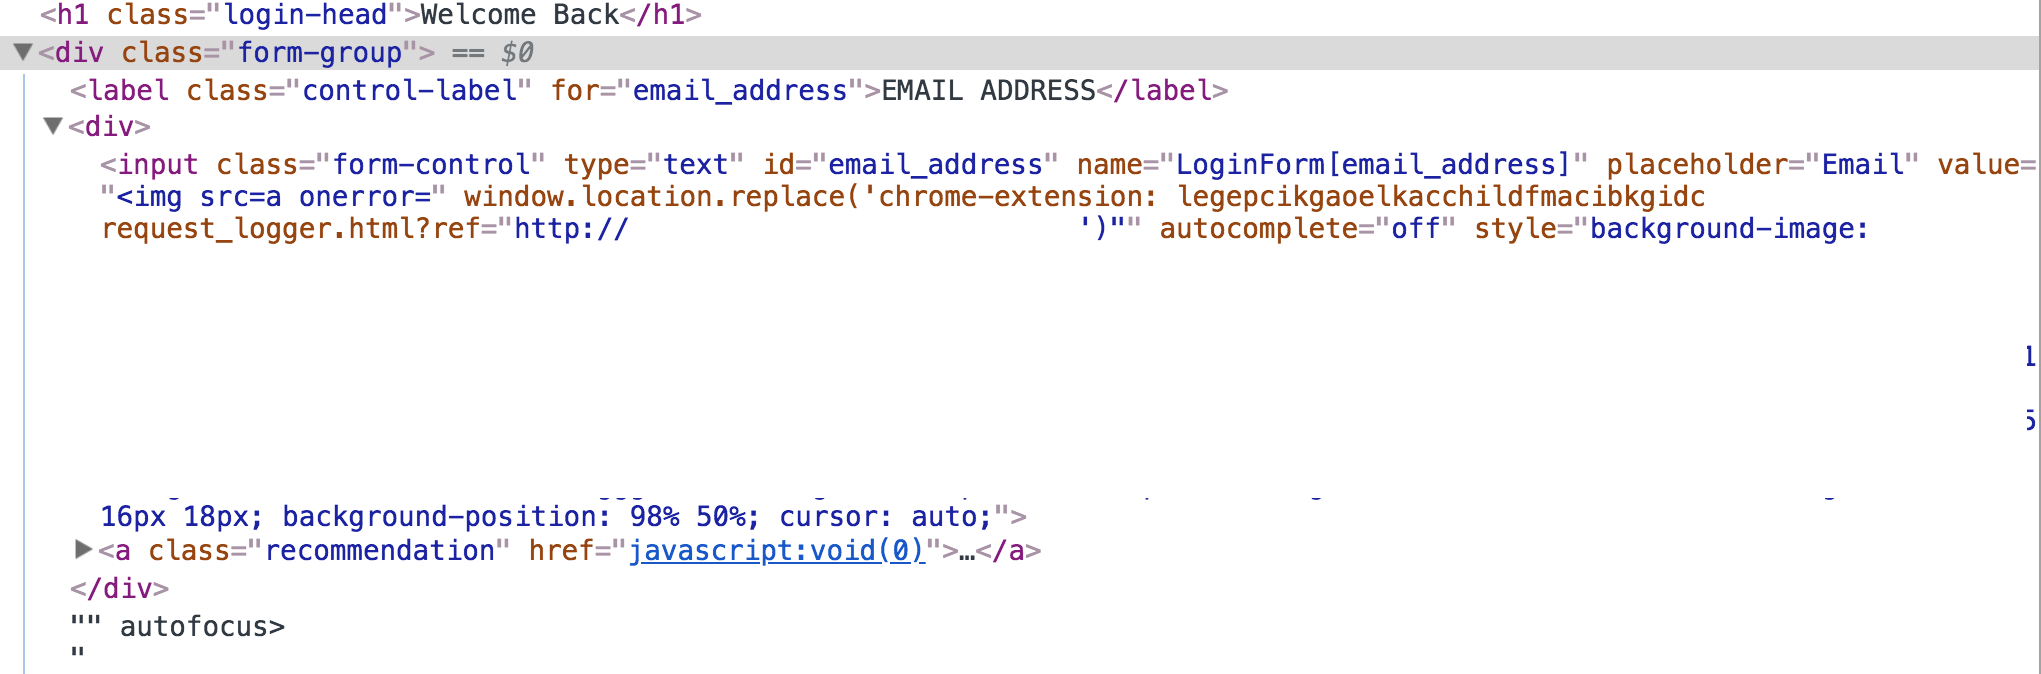
\includegraphics[width=\linewidth]{images/test_case_1/src_code_after.png}
	\caption{The source code of the login form after executing the attack (edited for anonymity).}
	\label{fig:src_code_after}	
\end{figure} 

Comparing the page source code before and after submitting the attack shows that before the attack, the \texttt{autofocus} attribute was immediately after the \texttt{value} attribute of the \texttt{email} input. The \texttt{value} attribute had no prior setting. We know that upon submission of a form, the \texttt{value} attribute of an input is changed to whatever the user has submitted. In this case, that value contained the \texttt{"} character. What seems to have happened is that the browser adds the quote characters to encapsulate the incoming value for this attribute (as they were not present before), but because that value contains quote characters of its own, these are not escaped, and thus cause a shift in attributes in the form input. That explains why we see the shift of the \texttt{autofocus} attribute towards the bottom of the code section in Figure \ref{fig:src_code_after}. \\

Armed with this knowledge, we can now play the role of a potential attacker and experiment with different inputs to try and generate an exploit. Before proceeding and potentially wasting time on attempting exploits that may not work, we enable Passive Mode and have a quick look at whether using this form tells us anything about the headers being set on the page. Figure \ref{fig:passive_analysis} only alerts us to the lack of a \texttt{Content-Security-Policy}. \\

\begin{figure}[h!]
	\centering
	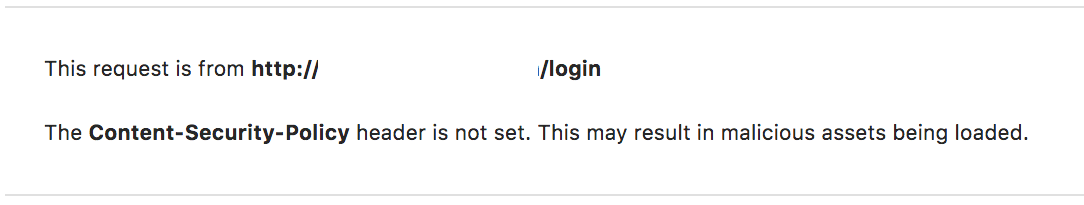
\includegraphics[width=\linewidth]{images/test_case_1/passive_analysis.png}
	\caption{Analysing the website using the Passive Mode of the extension reveals that of the security headers, only the \texttt{Content-Security-Policy} header hasn't been set. }
	\label{fig:passive_analysis}	
\end{figure} 

This saves a website pentester some time - they may skip attempting to craft an XSS exploit as an example because the \texttt{X-XSS-Protection} header has already been set, which makes this difficult unless they know specific ways to bypass browser XSS protection. This for example means that we cannot make use of inline Javascript attributes (such as \texttt{onclick}), but does not prevent us from using other HTML attributes. We can attempt to craft a form which looks similar to the present one, but with a different result from submission - we try and trick a user into downloading a file from an external source. \\

To start this, we want to introduce our own elements into the form, but we know we can't directly remove elements from that form, since we don't have access to Javascript to remove this. We can however shift the contents of the page, just as we have inadvertently done with the \texttt{autofocus} attribute. Following this principle, we try and shift the current contents of the form as far down the page as we can. We do this by injecting prematurely closing DOM tags in the email input. We try the following attack:

\begin{center}
	\texttt{"></form></section>}
\end{center}

This produces the webpage as shown in Figure \ref{fig:attack_form_1}. That figure shows what is immediately visible to the user. However, if the user were to scroll down in the page, they would see the remaining contents of the form, which have simply been displaced further down the page - as seen in Figure \ref{fig:scroll_attack_1}. \\

\begin{figure}[h!]
	\centering
	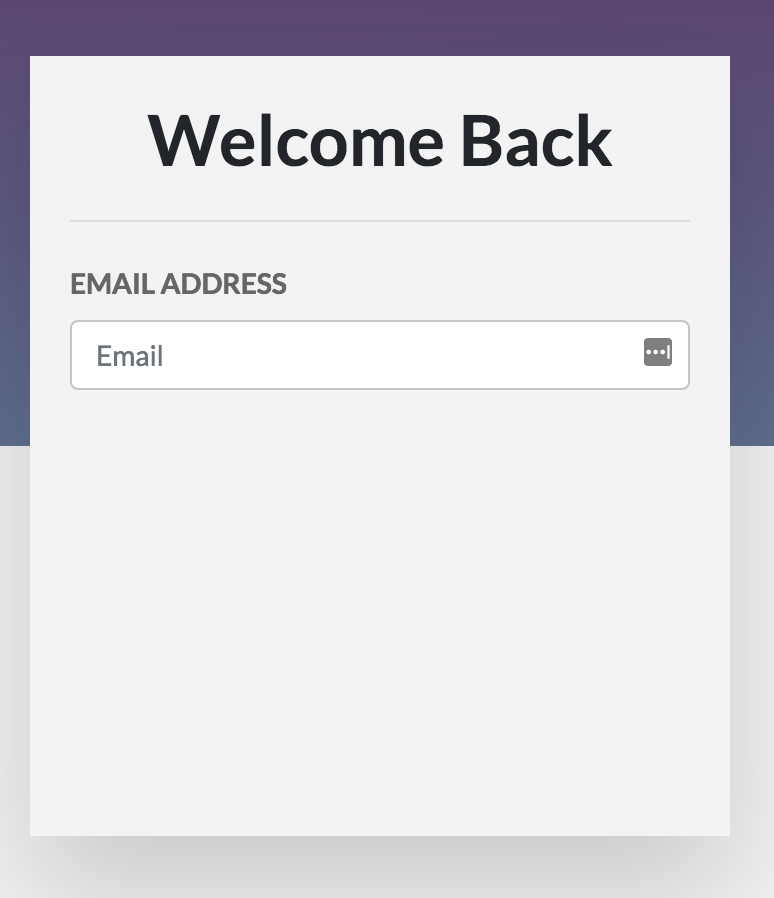
\includegraphics[width=0.6\linewidth]{images/test_case_1/attack_form_1.png}
	\caption{This is the resulting page from prematurely closing DOM tags. }
	\label{fig:attack_form_1}	
\end{figure} 


\begin{figure}[h!]
	\centering
	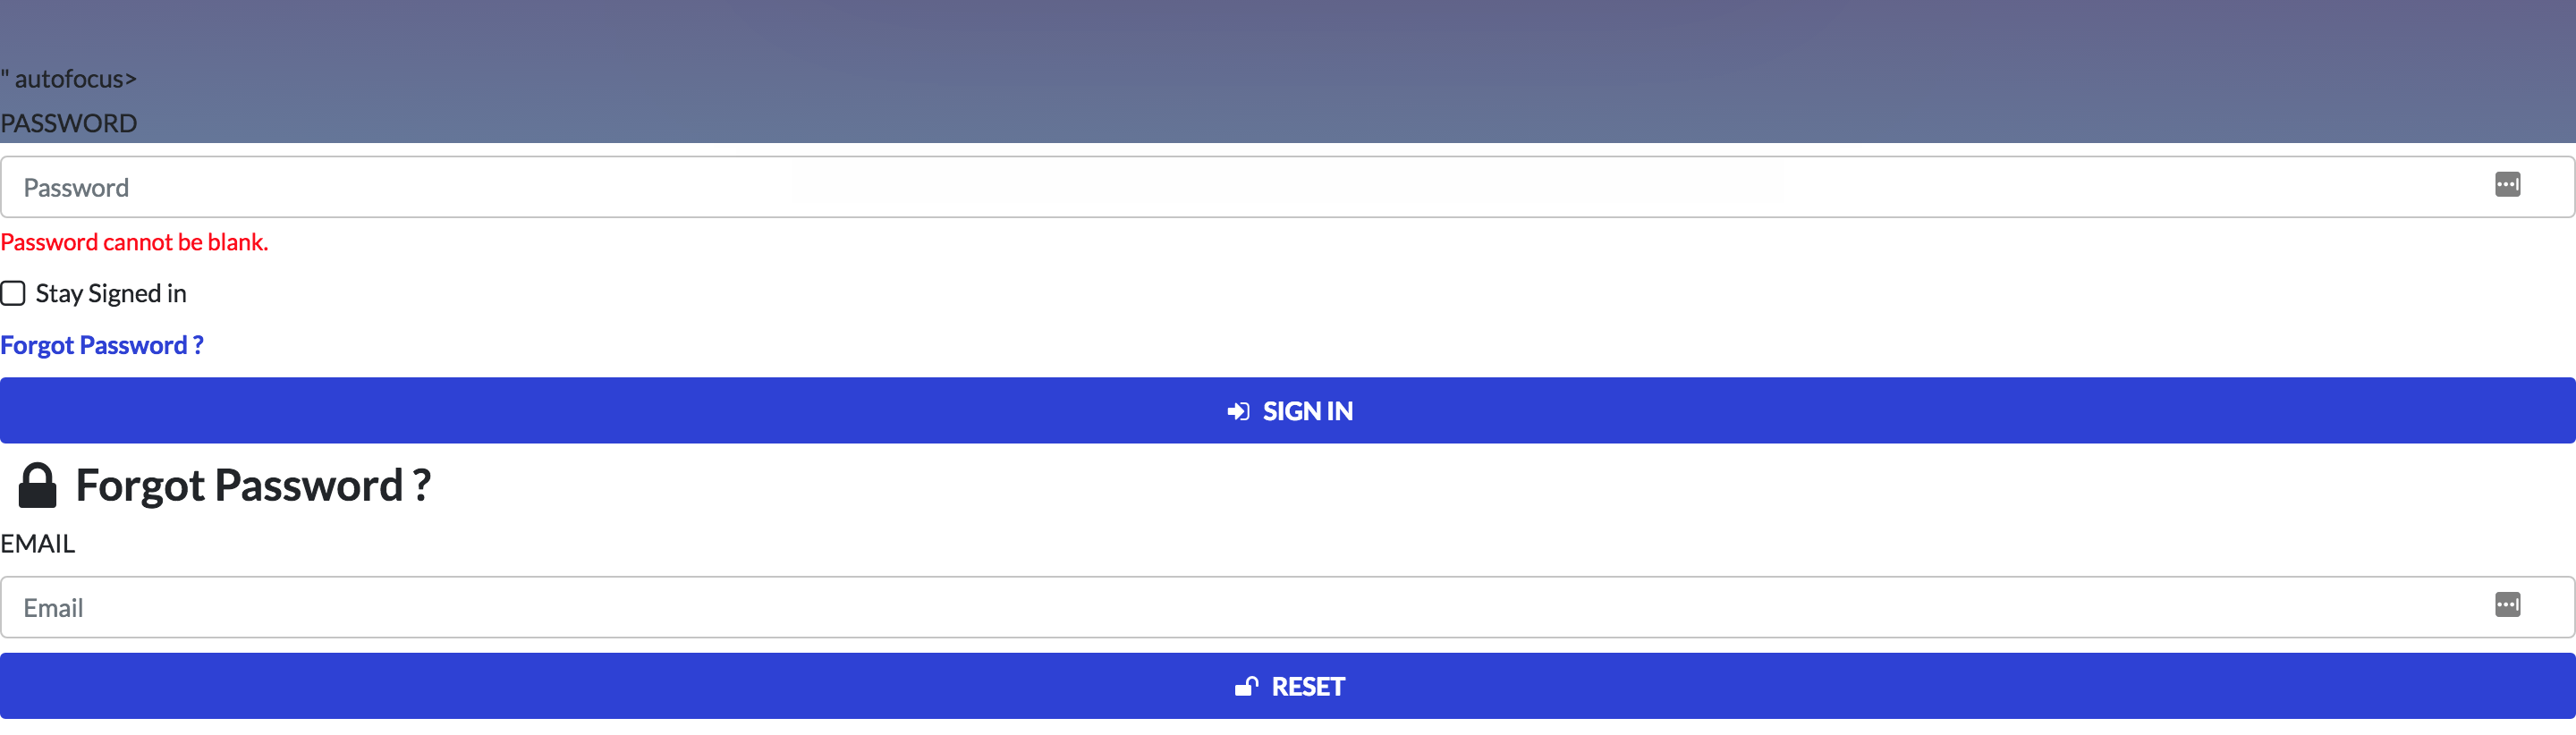
\includegraphics[width=\linewidth]{images/test_case_1/scroll_attack_1.png}
	\caption{Scrolling down the page reveals the "missing" contents of the form to submit.}
	\label{fig:scroll_attack_1}	
\end{figure} 

Now that we have figured out how to make it seem as if the contents of the form are broken, we can add in our own elements to this form. Since our goal is to make the user inadvertently download a file, we simply need the user to click somewhere with a link to that file. It is tempting to attempt to steal their password and email address by making the form submit to a website we control, thus including these details in the request. However, changing the \texttt{action} attribute of the form to a value we control would be picked up by the browser's XSS auditor, and thus disabled. To fulfill our goal, we thus want to inject an anchor (\texttt{<a>}) tag to replace the \textit{Submit} button on the form. In order to start the download of the file, we make the \texttt{href} attribute of this tag link to a webpage where this file is hosted. For the purposes of this example, we have prepared a file to be hosted at a website we control, with a file extension we know Chrome automatically downloads, \texttt{.dmg} (some file extensions such as \texttt{.pdf} open up special browser features to open or read the file in question). Since the attacks are being executed on a macOS, this file type is considered an executable, and is downloaded automatically. Obviously, the contents of this file are harmless, we are only showing a proof-of-concept in terms of exploits. \\

Thus, with a bit of trial and error, as well as adding some custom CSS as part of the injection, we can arrive at the exploit code necessary to craft a form which looks as though it could be part of the legitimate website. The exploit code is included in full in the Appendix \ref{exploitCode}. Injecting this code into the \textit{Email address} field of the form generates a form as shown in Figure \ref{fig:fake_form_anon}. \\

\begin{figure}[h!]
	\centering
	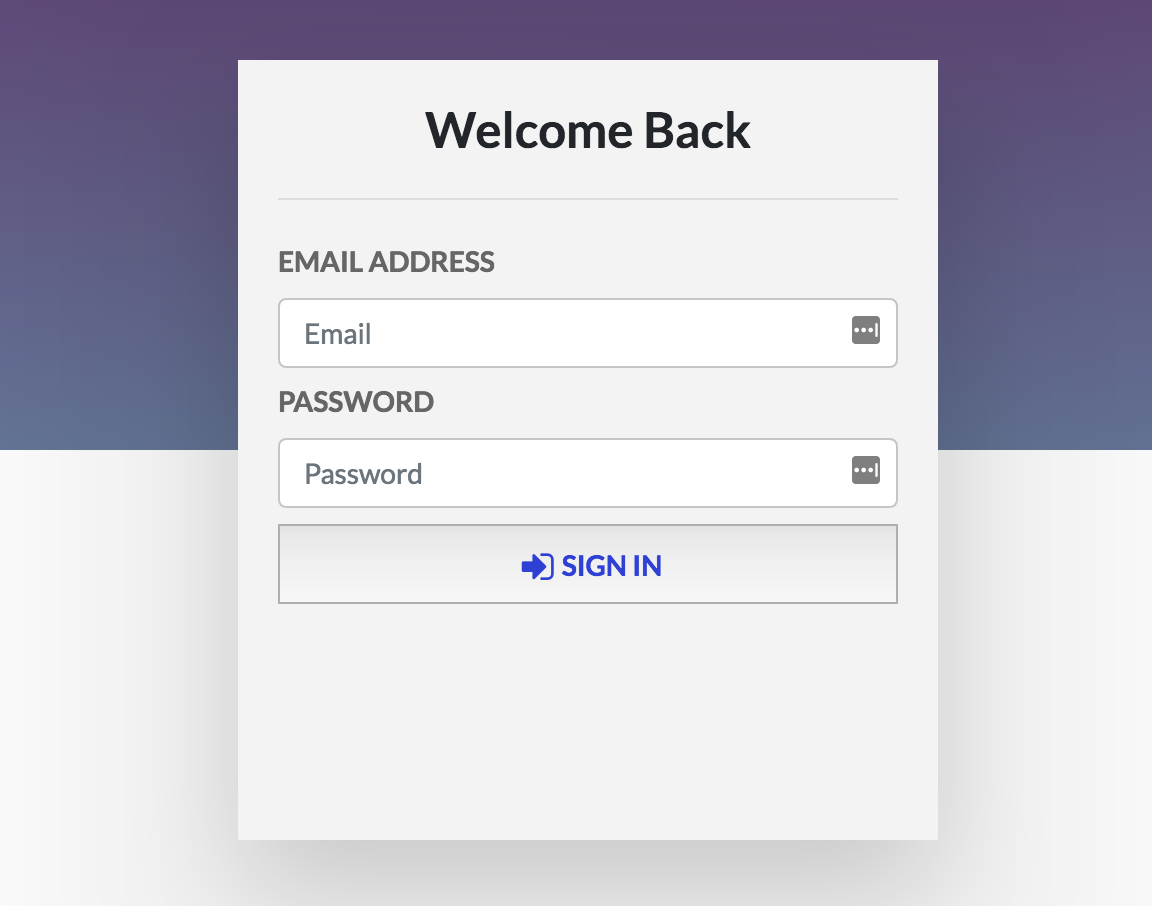
\includegraphics[width=0.8\linewidth]{images/test_case_1/fake_form_anon_cropped.png}
	\caption{Exploiting the injections in this form allow us to create a customized form of our own, where the Submit "button" downloads a file from an external website.}
	\label{fig:fake_form_anon}
\end{figure} 

As before, if the user is wary enough to recognise that some of the aspects of this form look different to the original form (such as the missing \textit{Stay signed in} and \textit{Forgot Password} buttons), they may be more prudent as to using this form as usual. Although the original website does not immediately offer scrolling (because the content is finished before the page requires any scrolling), if the user happens to scroll in the malicious form they may quickly identify that something is wrong with the page; as before, the contents have been displaced further down the page, and can be seen when the user scrolls down. \\

Should the user submit this form by pressing the \textit{Sign in} button, the download is instantly initiated, and as we see in Figure \ref{fig:download_completed}, \texttt{EVIL.dmg} is downloaded. \\

 \begin{figure}[h!]
 	\centering
 	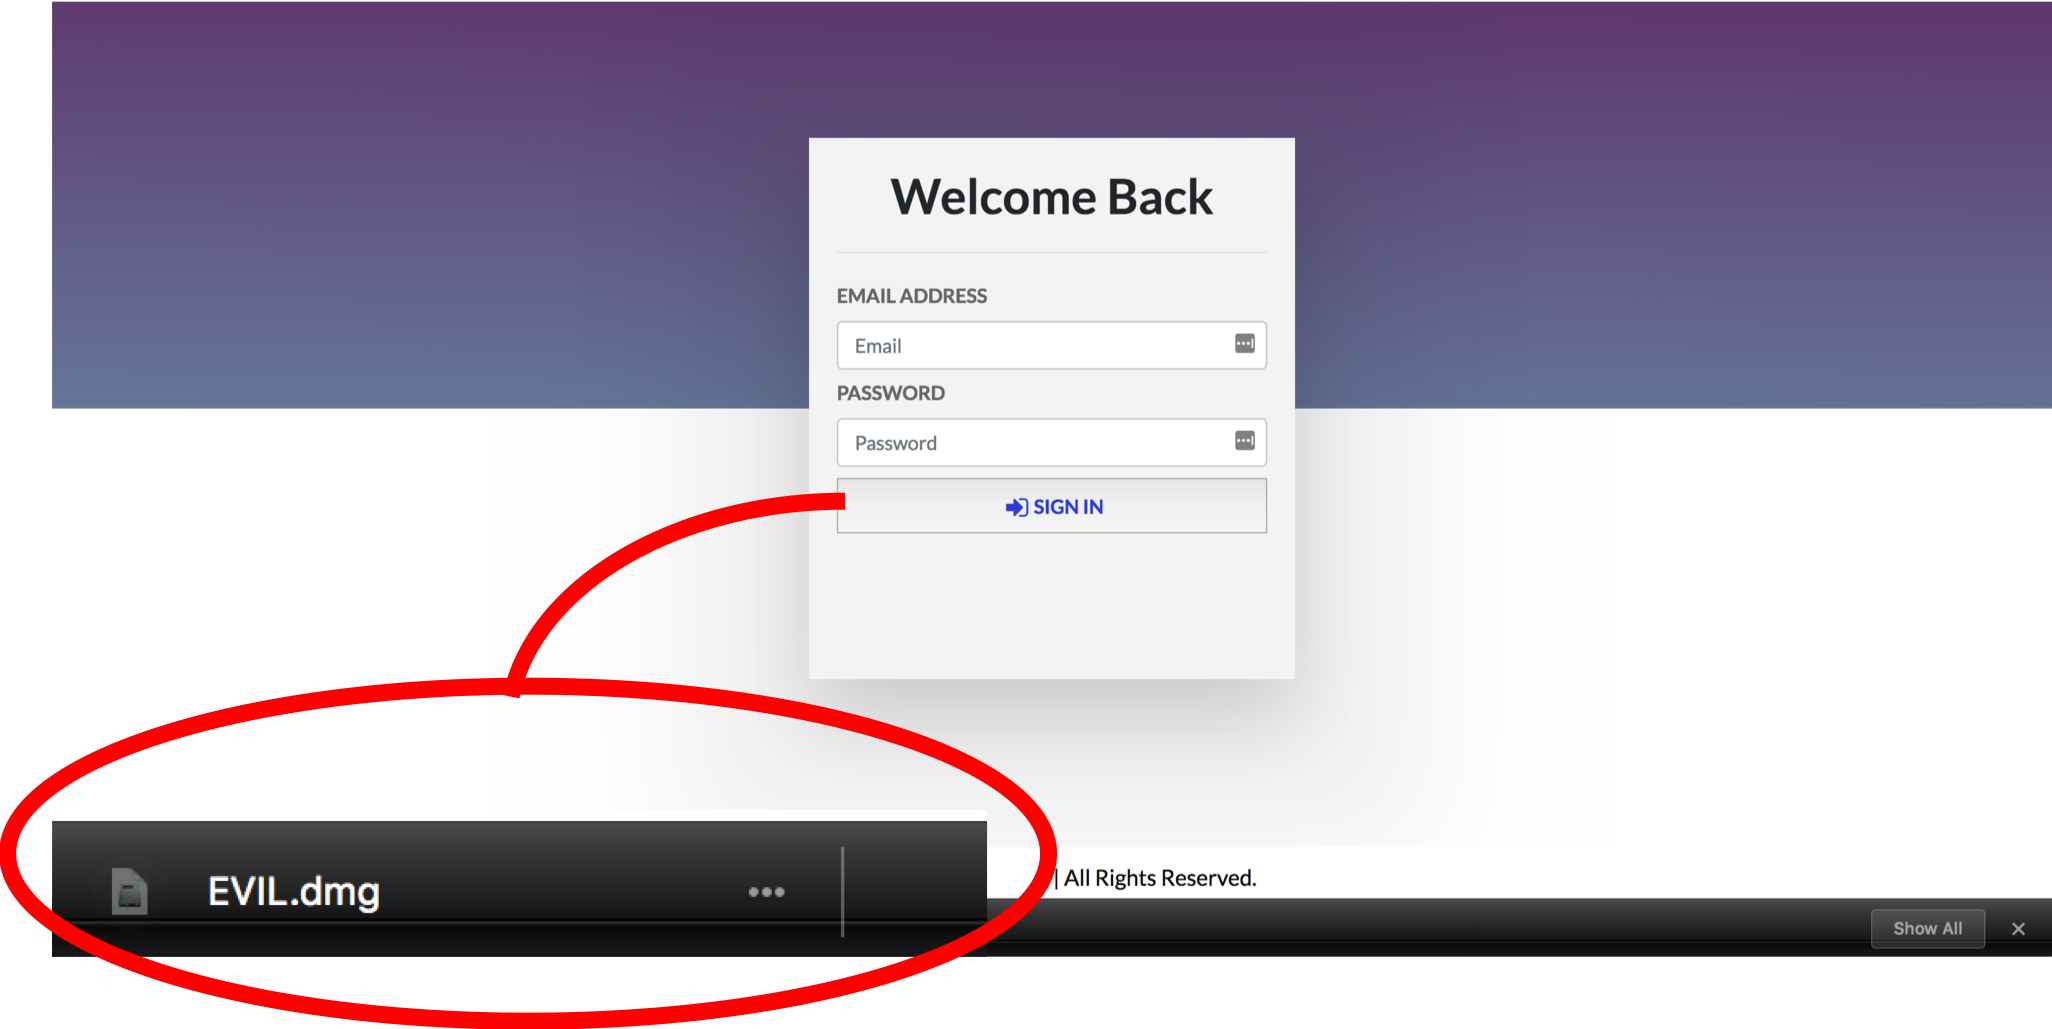
\includegraphics[width=0.8\linewidth]{images/test_case_1/downloaded_evil.png}
 	\caption{The download is instantly initiated after pressing the \textit{Sign in} button. This could pose a security risk if the contents of \texttt{EVIL.dmg} were malicious.}
 	\label{fig:download_completed}
 \end{figure} 





















